%% The openany option is here just to remove the blank pages before a new chapter
\documentclass[11pt,openany]{book}
\usepackage[utf8]{inputenc}
\usepackage[utf8]{vietnam}
\usepackage{subcaption}
\usepackage{graphicx}
\usepackage{kantlipsum}
\usepackage{amsfonts}
\usepackage{amsmath}
\usepackage{float}
\usepackage{algorithm}
\usepackage{algorithmic}
\usepackage{hyperref}
\usepackage{tabularx}
\usepackage{diagbox}
\usepackage{slashbox}
\usepackage{lscape}
\usepackage{multirow}
\usepackage{longtable}
\usepackage{biblatex}
\addbibresource{mybib.bib}
\title{Communicating Multi-UAV System for cooperative SLAM-based Exploration}

\usepackage{pagenote}
\setcounter{chapter}{0}

%% End notes to be printed as sections at the
%% end of each chapter.
\renewcommand*{\notedivision}{\section*{\notesname}}
\renewcommand*{\pagenotesubhead}[1]{}


%%%%%%%%%%%%% For customising the endnote markers. Comment these out if you don't want them.
% To prefix each note number with the chapter number
\renewcommand{\thepagenote}{\thechapter-\arabic{pagenote}}

% To have a slightly different formatting for the endnote numbers in the text -- smaller text, sans-serif, square brackets
\renewcommand\notenumintext[1]{\space{\footnotesize\sffamily[FN-#1]}}

% To have a slightly different formatting for the endnote numbers in the notes section. Just the square brackets and sans-serif; normal size.
\renewcommand\notenuminnotes[1]{{\sffamily[FN-#1] }}

% If you want a different name/heading for the end notes
\renewcommand{\notesname}{End Notes}
%%%%%%%%%%%%% End customisation

%% THIS LINE IS MANDATORY
\makepagenote

\begin{document}
\begin{titlepage}
    \begin{center}
        \small
        TRƯỜNG ĐẠI HỌC BÁCH KHOA HÀ NỘI\\
        \vspace{0.2cm}
        \LARGE
        \textbf{VIỆN ĐIỆN TỬ - VIỄN THÔNG}\\
        \vspace{1.5cm}
        
\includegraphics[scale=0.3]{assets/logo.png}\\
        \vspace{1.5cm}
        \LARGE
        BÁO CÁO GIỮA KỲ\\
        \vspace{0.5cm}
        \Huge
        \textbf{ĐIỆN TỬ TƯƠNG TỰ II \\ DỊCH TÀI LIỆU}
        \vspace{1cm}
        \Large
        \begin{center}
            \begin{tabular}{ l l }
                \textbf{Nhóm}        & 49            \\
                \textbf{Sinh viên 1} & Tạ Hoàng Việt \\
                                     & 20172916      \\
                \textbf{Sinh viên 2} & Hồ Huy Hoàng  \\
                                     & 20172581
            \end{tabular}
        \end{center}
        \vspace{1cm}
        \normalsize
        Hà Nội, 06/2021
    \end{center}
\end{titlepage}
\tableofcontents
\listoffigures
\listoftables
\newpage
\thispagestyle{plain}
\addcontentsline{toc}{chapter}{Introduction}
\begin{center}
    \Huge
    \textbf{Introduction}
\end{center}
% TODO: add introduction here
\chapter{Coordinated exploration}
\section{Introduction}
The exploration and mapping of large areas is an active field of research in aerial robotics. It consists in constructing a 3D model representation of the workspace as robots progress within it. Recently, the key subject in the exploration problem is the cooperative deployment of fleet of robots that promise enhanced performances compared to single robot exploration.\\\\
In this chapter, we address the problem of cooperative exploration strategies with no a- priori knowledge of the environment. We will try to answer the question: Where should each robot move next?
\section{Related work}
Recently, several works have proposed solutions for exploration using multi-robot teams to reduce the mission time and to increase the scalability \cite{bautin2012strategie}, \cite{jensen2013rolling}, \cite{yan2014team}. Hence, the challenge is to have an efficient cooperation among the agents in the fleet while maintaining communication \cite{rooker2007multi}. For that, existing approaches can be centralized, that is, one robot in the fleet is responsible for assigning targets \cite{burgard2000collaborative}. In \cite{schmuck2017multi}, a central server with increased computational resources is adopted to receive, treat, optimize and send back information to other robots. Other works, such as \cite{yuan2010cooperative},\cite{sheng2006distributed}, use distributed approaches where each robot chooses its own target. Another trend is to switch from individual to cooperative exploration behavior when robots are not able to converge to a local minimum at a satisfying rate \cite{wu2012robust}. In \cite{konolige2003map}, authors propose to consider four possibilities taking into account robots’ interactions in order to construct a distributed map. The situations involved are: no interaction (robots are not within each others’ communication range), hypothesis generation (there is an interaction between the robots but they do not know their respective location), hypothesis verification (there is an interaction between the robots and they propose an hypothesis about their location), and coordinated exploration (there is an interaction between robots and they do share their maps).
\subsection{Robot-to-target assignment}
The mapping algorithm is performed while a robot attempts to reach a target. So, for an effective environment mapping, the target should be chosen carefully. There is a wide variety of goal assignment strategies to affect one robot to a target. The majority of them are centralized and use a cost function to compute the utility of reaching a target.\\\\
In the greedy assignment \cite{yamauchi1998frontier}, each robot chooses a target depending on its cost function without coordinating with other robots. Hence, one target can be visited by different robots. To solve this issue, already chosen targets can be discarded before being considered for assignment by others using Broadcast of Local Eligibility (BLE) \cite{werger2000broadcast} also called Iterative Assignment. But, this method does not necessarily produce the optimal solution since it depends on the order of robots.\\\\
The K-means method \cite{solanas2004coordinated} consists in dividing the environment to explore into regions of the same number of robots, then, assigning one robot to the closest region where it will choose a target from the frontiers depending on a cost function.\\\\
The Hungarian method \cite{deb1999multi} proposed by \cite{kuhn2005hungarian}, solves the worker- task assignment written in the form of $n \times n$ matrix $C$ where $c_{i,j}$ is the cost of the task $j$ assigned to the worker $i$. The optimal assignment is found with time complexity $O(n^3)$. This algorithm requires that the number of workers is equal to the number of tasks which cannot be guaranteed. Else, imaginary robots or targets can be added to satisfy the assumption, and skipped later in the selection.\\\\
Authors in \cite{nanjanath2006dynamic} present an auction-based method to assign tasks to a group of robots. The distribution of tasks is accomplished by means of a first-price reverse auction which means that the auctioneer is the buyer. One task is auctioned one at a time by priority. Then, the auctioneer selects the best bid and assigns the task to the corresponding bidder. The algorithm is well adapted to dynamic environments, where unexpected obstacles might prevent a robot from reaching its target.\\\\
In \cite{zhao1996genetic}, \cite{leigh2007using}, a genetic algorithm is used to optimally assign robot to tasks. It is an NP-hard problem since it is considered as a generalized two- dimensional multi-type bin packing problem.\\\\
Authors in \cite{faigl2012goal} present a new approach called Multiple Traveling Salesman Problem (MTSP) for robot-to-target assignment in multi-robot exploration problem. It consists in clustering an environment, determining the cost of TSP distance for each pair of robot cluster, assigning goals from non empty cluster, and finally fixing goals for empty clusters. This approach was compared with greedy, iterative and Hungarian method. The MTSP presents competitive results regarding the total computational requirements and the increasing number of robots.\\\\
In \cite{kulich2015comparison}, a comparison of some assignment strategy used for multi- robot system is done. The compared strategies include Hungarian method, Greedy, BLE method and K-means clustering. Results show that Hungarian method outperforms other approaches in majority of cases. Unlike the Hungarian method, the iterative assignment can be implemented in a distributed environment. Also the Hungarian methods are computationally heavy compared with the simple greedy algorithm which is preferred in applicable scenario.
\subsection{Utility function}
Most of the robot-to-target assignments are based on an utility function that defines the benefits that a robot have to reach this target, taking into account the mission’s aim \cite{burgard2000collaborative}. The work proposed in \cite{benavides2016multi} presents a new utility function that takes into account the traveling cost to the target and the connectivity utility. This allows a trade off between minimizing the amount of exploration time and the connectivity. To speed up velocity, authors in \cite{cieslewski2017rapid} propose a rapid frontier selection technique to select goals from the robot’s field of view. This approach minimizes the overall mission time by minimizing the change in velocity of the robot. Nonetheless, this approach increases the total path length traveled. In \cite{heng2015efficient}, maximizing the reconstructed model is favored over the mission time. Furthermore, the proposed approach solves simultaneously exploration and coverage problems in order to maximize the completeness of the reconstructed model. Whereas in \cite{simmons2000coordination}, the aim is the maximization of the utility of targets that minimizes the potential for overlap in information gain amongst members of the fleet. The utility of reaching a target depends basically on the aim of the mission while taking into account some additional constraints such as time, completeness of the map, limited sensor and communication range, or number of robots.
\section{Proposed exploration strategy}
\subsection{Overview}
In a Multi-UAV system, the exploration strategy needs to be cooperative to maximize the efficiency. The main objective proposed here, is to cooperatively choose specific regions to be simultaneously explored using a frontier-based approach. Commonly, this is done by selecting candidate targets and assigning them to each robot in an optimized manner. Figure \ref{fig:3.1} shows the proposed pipeline exploration process performed by each UAV.
\begin{figure}[H]
    \centering
    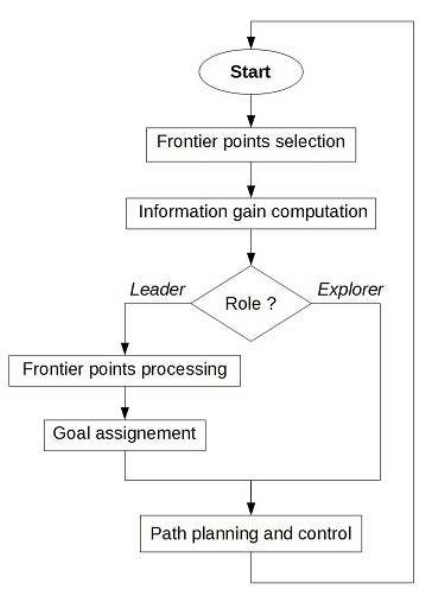
\includegraphics[scale=0.6]{assets/3_1.png}
    \caption{Proposed exploration process pipeline.}
    \label{fig:3.1}
\end{figure}
Each UAV selects the frontier points of its constructed local map during the SLAM step. Then, it computes the corresponding information gain of these points. If the UAV’s role is an \textit{explorer}, it would passively wait until receiving instructions; else, if it acts as a \textit{leader}, it would process the collected frontier points, and would assign a target to each robot in the group. Given a target, UAVs will plan a specific path to reach it.\\\\
During these steps, the map structure evolves from a projected 2D grid map obtained from the localization and mapping module, through frontier points during the frontier selection process, then candidate targets during the frontier processing step, to a final set of selected targets to reach. The evolution of the map structure is illustrated in Figure \ref{fig:3.2}. Algorithm \ref{alg:3.1} describes the main steps performed during the exploration.
\begin{algorithm}
    \caption{Exploration strategy for coordinated Multi-UAV}
    \label{alg:3.1}
    \begin{algorithmic}[1]
        \STATE From cell $\mathbf{l}_l \in \mathcal{L}$, select frontier points $\mathbf{f}_{i,j} \in \mathcal{F}$ and compute their respective information gain $\mathit{\mathbf{I}}(\mathbf{f}_{i,j})$.
        \STATE Process frontier points $\mathbf{f}_{i,j}$ to get candidate goals $\mathbf{t}_k \in \mathcal{G}$ (See Algorithm \ref{alg:3.2})
        \STATE Assign UAV$_i$ with target $k$ (See Algorithm \ref{alg:3.2}).
        \STATE Send targets to the corresponding robots.
    \end{algorithmic}
\end{algorithm}
\begin{figure}[H]
    \centering
    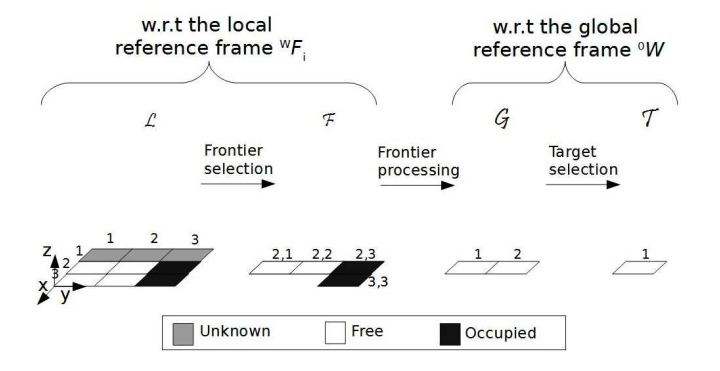
\includegraphics[scale=0.4]{assets/3_2.png}
    \caption{Map structure evolution during the exploration process: From 2D cells $\mathcal{L}$ to 2D frontier cells $\mathcal{F}$ to candidate frontier cells/points $\mathcal{G}$ (candidate targets) to 2D target cells/points $\mathcal{T}$.}
    \label{fig:3.2}
\end{figure}
\subsection{Frontier points selection}
The frontier selection process is used to define the frontiers of regions bounded by obstacles or unknown spaces (See Figure \ref{fig:3.3}).
\begin{figure}[H]
    \centering
    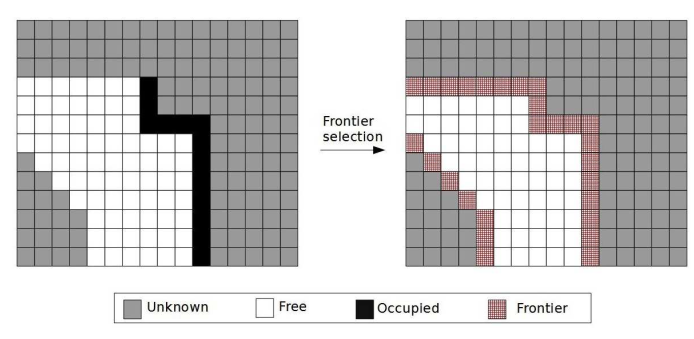
\includegraphics[scale=0.4]{assets/3_3.png}
    \caption{Frontier cells/points selection of a 2D occupancy grid map.}
    \label{fig:3.3}
\end{figure}
The frontier cells $\mathbf{f}_{i,j} \in \mathcal{F}$ are selected from the set of cells $\mathcal{L}(\mathcal{F}\subset \mathcal{L})$ such that they are either:
\begin{itemize}
    \item Free $\mathbf{l}_f$ and adjacent to unknown.
    \item Labeled as occupied $\mathbf{l}_o$ . The Occupied cells $\mathbf{l}_o$ are considered as frontier cells to be able to perform frontier processing in the next step. They could not be chosen as target and will be discarded later.
\end{itemize}
In Figure \ref{fig:3.2}, the frontier cells are: $\mathbf{l}_f(2,1)$,$\mathbf{l}_f(2,2)$ , $\mathbf{l}_f(2,3)$, and $\mathbf{l}_f(3,3)$. Thus, for a cluster $\mathcal{C}$ containing UAV$_i$ , the frontiers are:
\begin{equation} \label{eq:3.1}
    \mathcal{F}=\{\mathbf{f}_{i,1}(2,1),\mathbf{f}_{i,2}(2,2),\mathbf{f}_{i,3}(2,3),\mathbf{f}_{i,4}(3,3)\}
\end{equation}
\subsection{Information gain computation}
In frontier-based exploration approaches, only cells adjacent to unknown ones may be defined as candidate frontier points and are likely to be chosen as targets. Thereby, the information gain is associated to each of them in order to estimate the utility of reaching each frontier. This corresponding information gain can be defined in different manners depending on the mission purpose. Authors in \cite{burgard2005coordinated} propose to use a probability function to reduce an assigned constant value taking into account the relative distance to the UAV’s pose. This strategy is general and does not take into account the updated explored cells. The approach proposed in \cite{heng2015efficient} affects, to the information gain, the number of unknown and not occluded cells in the view frustum of the target. This method depends on the real estimate of information gained when visiting the considered pose. However, it requires more computation.\\\\
In the proposed strategy, the information gain is allocated so that it defines the amount of unknown cells surrounding the target (See Figure \ref{fig:3.4}). It is a non-metric value that counts the number of cells labeled as unknown l u from the 48 cells around the frontier point.
\begin{figure}[H]
    \centering
    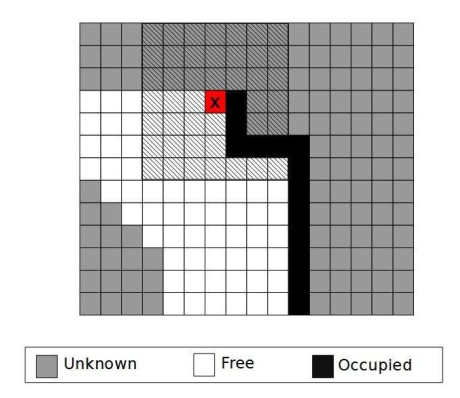
\includegraphics[scale=0.4]{assets/3_4.png}
    \caption{The information gain computation of a frontier point x (in red). The hatched cells represent the 48 surrounding cells of the frontier point \textbf{x}. The information gain of \textbf{x} is: $\mathbf{I}(x)=25$.}
    \label{fig:3.4}
\end{figure}
\subsection{Frontier points processing}
All frontier points $\mathbf{f}_{i,j} \in \mathcal{F}$ of UAV$_i$ in the cluster $\mathcal{C}$ with $i \in [1..n_c]$, are collected. Points in $\mathcal{F}$ are then processed using Algorithm \ref{alg:3.2} to get candidate frontier points considered as candidate targets $\mathbf{t}_k \in \mathcal{G}$ with $k \in [1..n_g]$ (See Figure \ref{fig:3.2})
\begin{algorithm}[H]
    \caption{Frontier processing algorithm.}
    \label{alg:3.2}
    \hspace*{\algorithmicindent} \textbf{Input:} Frontier points $\mathbf{f}_{i,j} \in \mathcal{F}$ of UAV$_i$ with $i \in [1..n_c]$. \\
    \hspace*{\algorithmicindent} \textbf{Output:} Candidate targets $\mathcal{G}$
    \begin{algorithmic}[1]
        \STATE $p_u=\cup_{i=1}^{n_c}\mathbf{f}_{i,j}$.
        \STATE $p_i=\cap_{i=1}^{n_c}\mathbf{f}_{i,j}$.
        \STATE $\mathcal{G}=p_u\setminus p_i$.
        \STATE Delete the obstacle frontier points $\mathbf{f}_{i,j}(x,y)=\mathbf{l}_o(x,y)$ from $\mathcal{G}$.
        \RETURN $\mathcal{G}$.
    \end{algorithmic}
\end{algorithm}
Figure \ref{fig:3.5} shows an example of frontier processing with two UAVs’ map to get the candidate targets. The obstacle frontier points $\mathbf{f}_{i,j}(x,y)=\mathbf{l}_o(x,y)$ – labeled as occupied – are only kept to compute the intersection of frontier points. Only the free frontier cells $\mathbf{l}_f$ can be considered as candidate target.\\\\
When using local frontier points instead of local maps, the frontier process replaces the map matching process where the aim is to clear overlapping areas. Hence, in the frontier processing step, the frontier points that belong to overlapping areas are cleared. Therefore, using frontier points allows important memory saving. To compute the frontier points that belong to the overlapped areas (Steps 1, 2 and 3 in Algorithm \ref{alg:3.2}), we propose two approaches with convex shapes and concave shapes assumptions.
\subsubsection{First approach: Convex shape map}
In this approach, map shapes are considered convex, which simplifies the intersection computation in Algorithm \ref{alg:3.3}. Figure \ref{fig:3.6} shows two examples of applying frontier processing algorithm while assuming convex shapes with two and three UAVs’ map.\\\\
This algorithm is relatively easy to apply, but results show that it does not perform well. The convex assumption leads to some false overlapped frontier points. Consequently, some unknown areas will not be visited since their corresponding points are removed and, thus, will not be assigned as a target.
\subsubsection{Second approach: Concave shape map}
In the second approach, we make the assumption of concave shapes for the UAVs’ map to compute their intersection in Algorithm \ref{alg:3.4}. Figure \ref{fig:3.7} shows two examples of applying frontier processing algorithm while assuming convex shapes with two and three UAVs’ map.
\begin{figure}[H]
    \centering
    \begin{subfigure}[H]{0.6\linewidth}
        \centering
        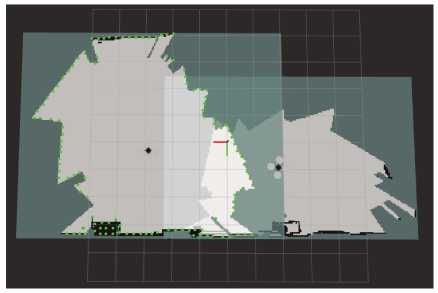
\includegraphics[width=\linewidth]{assets/3_5_a.png}
        \caption{{Frontiers $\mathbf{f}_{1,j}$ of UAV$_1$}}
        \label{fig:3.5a}
    \end{subfigure}
    \begin{subfigure}[H]{0.6\linewidth}
        \centering
        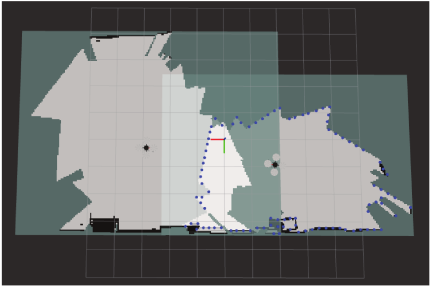
\includegraphics[width=\linewidth]{assets/3_5_b.png}
        \caption{{Frontiers $\mathbf{f}_{2,j}$ of UAV$_2$}}
        \label{fig:3.5b}
    \end{subfigure}
    \begin{subfigure}[H]{0.6\linewidth}
        \centering
        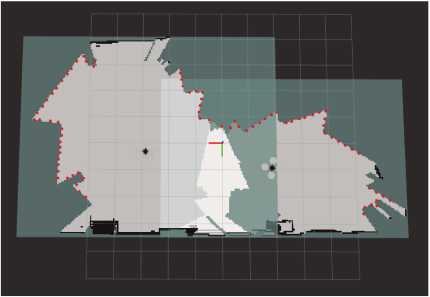
\includegraphics[width=\linewidth]{assets/3_5_c.png}
        \caption{{Candidate targets $\mathcal{G}$}}
        \label{fig:3.5c}
    \end{subfigure}
    \caption{Frontier points processing example: (a) and (b) represent the frontier points of UAV$_1$ and UAV$_2$, respectively. (c) represent the candidate targets. The process consists in removing frontier points that belong to overlapped areas, and those that are adjacent to obstacles.}
    \label{fig:3.5}
\end{figure}
\begin{algorithm}[H]
    \caption{Intersection computation algorithm with convex shapes assumption.}
    \label{alg:3.3}
    \hspace*{\algorithmicindent} \textbf{Input:} $Vect1, Vect2$ \\
    \hspace*{\algorithmicindent} \textbf{Output:} $Vect\_Final$
    \begin{algorithmic}[1]
        \FOR {$i \in Vect1$}
        \STATE $inf = 0, sup = 0$
        \FOR{ $j \in Vect2$}
        \IF {$Vect1(i).x < Vect2(i).x$}
        \STATE $inf++$;
        \ELSE
        \STATE $sup++$;
        \ENDIF
        \ENDFOR
        \IF {$inf>0$ and $sup>0$}
        \STATE $Vect\_inter.push\_back(Vect1(i))$
        \ENDIF
        \ENDFOR
        \FOR{$i \in Vect\_inter$}
        \STATE $inf=0,sup=0$;
        \FOR{$j \in Vect2$}
        \IF {$|Vect\_inter(i).x-Vect2(i).x| <0.5$}
        \STATE $inf++$;
        \ELSE
        \STATE $sup++$;
        \ENDIF
        \ENDFOR
        \IF {$inf>0$ and $sup>0$}
        \STATE $Vect\_Final.push\_back(Vect\_inter(i))$
        \ENDIF
        \ENDFOR
    \end{algorithmic}
\end{algorithm}
\begin{figure}[H]
    \centering
    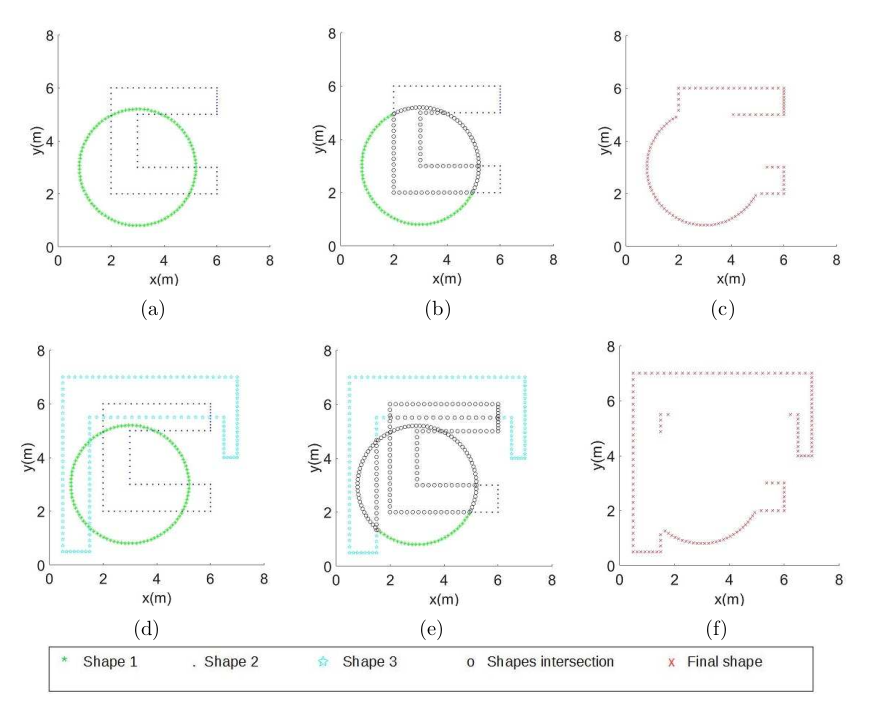
\includegraphics[scale=0.4]{assets/3_6.png}
    \caption{Frontier points processing wile assuming two convex map shapes in the first line and three in the second line. (a) and (d) represent two and three convex map shapes, respectively; (b) and (e) represent the frontier points in overlap (intersection); and (c) and (f) represent the obtained frontier points after processing (final shape).}
    \label{fig:3.6}
\end{figure}
\begin{algorithm}[H]
    \caption{Intersection computation algorithm with convex shapes assumption.}
    \label{alg:3.4}
    \hspace*{\algorithmicindent} \textbf{Input:} $Vect1, Vect2$ \\
    \hspace*{\algorithmicindent} \textbf{Output:} $Vect\_Final$
    \begin{algorithmic}[1]
        \FOR {$i \in Vect1$}
        \STATE $inf = 0, sup = 0$
        \FOR{ $j \in Vect2$}
        \IF {$Vect1(i).x < Vect2(i).x -0.5$}
        \STATE $inf++$;
        \ELSIF {$Vect1(i).x>Vect2(i).x+0.5$}
        \STATE $sup++$;
        \ELSE
        \STATE $eq++$;
        \ENDIF
        \ENDFOR
        \IF {$inf>0$ and $sup>0$ or $eq>0$}
        \STATE $Vect\_inter.push\_back(Vect1(i))$
        \ENDIF
        \ENDFOR
        \FOR{$i \in Vect\_inter$}
        \STATE $inf=0,sup=0, eq=0$;
        \FOR{$j \in Vect2$}
        \IF {$|Vect\_inter(i).y-Vect2(i).y| <0.5$}
        \IF {$Vect\_inter(i).x<Vect2(i).x-0.5$}
        \STATE $inf++$;
        \ELSIF {$Vect1(i).x>Vect2(i).x+0.5$}
        \STATE $sup++$;
        \ELSE
        \STATE $eq++$;
        \ENDIF
        \ENDIF
        \ENDFOR
        \IF {($inf>0$ and $sup>0$) or $eq>0$}
        \STATE $Vect\_Final.push\_back(Vect\_inter(i))$
        \ENDIF
        \ENDFOR
    \end{algorithmic}
\end{algorithm}
\begin{figure}[H]
    \centering
    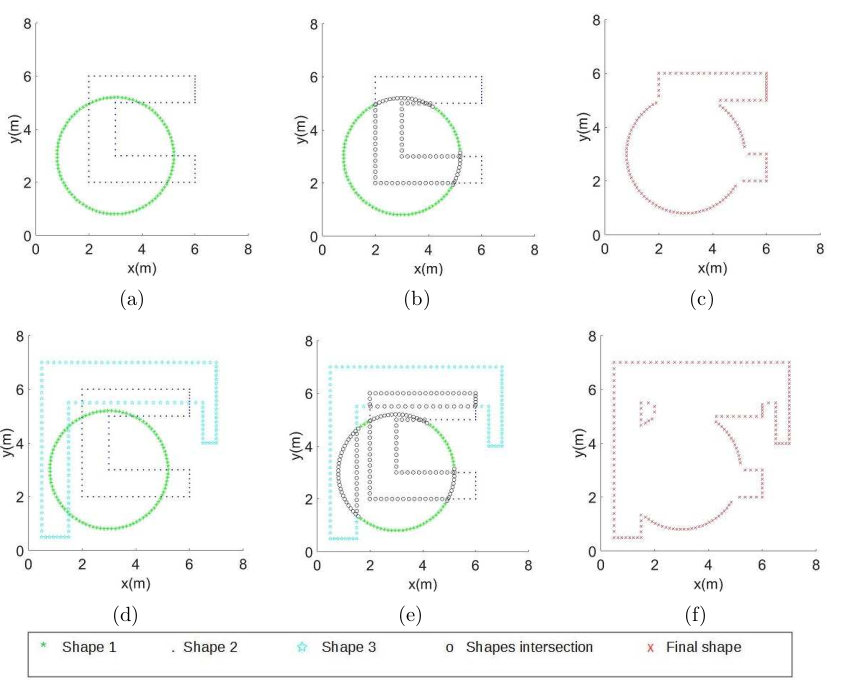
\includegraphics[scale=0.4]{assets/3_7.png}
    \caption{Frontier points processing wile assuming two concave map shapes in the first line and three in the second line. (a) and (d) represent two and three convex map shapes, respectively; (b) and (e) represent the frontier points in overlap (intersection); and (c) and (f) represent the obtained frontier points after processing (final shape).}
    \label{fig:3.7}
\end{figure}
Results show that only the frontier points within overlapping areas are removed. Even if some ambiguous frontier points are located within/inside the global shape – which can be confusing –, they are not deleted. This algorithm, assuming concave shapes, performs better than the previous one that assumes convex shapes. Hence, for the frontier processing, the shape of local maps are assumed concave.
\subsubsection{Utility function}
The proposed utility function in Eq. \ref{eq:3.2} aims to simultaneously increase the explored area rate and to reduce the distance of each UAV to its corresponding target. The function also considers the average of distances between each robot in the group and this target in order to maximize distances among robots.
\begin{equation}
    \mathbf{U}(UAV_i,t_j)=\mathbf{I}(t_j)exp(-\lambda.(dmin(\mathbf{P}_i,\mathbf{t}_j)+\frac{n_c-1}{d_{tot}})),
\end{equation}
where UAV i is the considered robot, $\mathbf{t}_j \in \mathcal{G}$ and $\mathbf{I}(\mathbf{t}_j)$ are respectively the candidate target and its corresponding information gain, $\lambda \in [0,1]$ is a trade-off parameter, $n_c$ is the number of UAVs in the cluster $\mathcal{C}$, and $d_{tot} = \sum_{k=1, k\neq i}^{n_c}(dmin(\mathbf{P}_k),\mathbf{t}_j) $ is the sum of the minimum distance from UAV$_k$'s pose $\mathbf{P}_k$ to the candidate target $j$. The proposed utility function is inspired from \cite{heng2015efficient} and it has been presented in our works \cite{mahdoui2017cooperative},\cite{mahdoui2018cooperative}. This function performs a trade-off between rapid exploration and a precise filling the map using a tuning parameter $\lambda$. From Figure \ref{fig:3.8}, we can notice that the larger $\lambda$, the less important the distance $d_{tot}$. Thus, a precise filling is favored over rapid exploration and vice versa.\\\\
Regarding the Multi-UAV case, the utility function is based on the average of neighbors distances. As shown in Figure \ref{fig:3.8}, with an information gain of $\mathbf{I}(\mathbf{t}_j)=25$ and three UAVs in the cluster $(n_c=3)$; an increasing distance of UAV to the target will reduce the utility function. Whereas, the larger the average distance from other UAVs w.r.t. to the target, the more the utility. So the function tends to choose the closest target to the considered UAV; but at the same time, the farthest one from the others.\\\\
In the case of a single UAV, the utility function (See Eq. \ref{fig:3.3}) tends to choose the closest target with the maximum of information gain:
\begin{equation}
    \mathbf{U}(UAV_i,\mathbf{t}_j)=\mathbf{I}(\mathbf{t}_j)exp(-\lambda.(dmin(\mathbf{P}_j,\mathbf{t}_j))),
\end{equation}
The parameter $d_{tot} = \sum_{k=1, k\neq i}^{n_c}(dmin(\mathbf{P}_k,\mathbf{t}_j)) $ represents the sum of the minimum distance between the target $\mathbf{t}_j$ and the neighbors’ poses $\mathbf{P}_k$ with $k \in [1..n_c]\setminus i$. So, if $\mathbf{t}_j$ has neighboring UAVs that are too far, the utility function will increase, so t j is more likely to be chosen.\\\\
The aim in the utility function is to maximize $d_{tot}$ . We distinguish two cases where $d_{tot}$ can be too close to zero or equal to it:
\begin{figure}[H]
    \centering
    \begin{subfigure}[H]{0.4\linewidth}
        \centering
        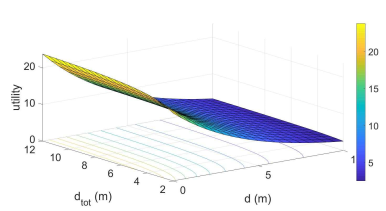
\includegraphics[width=\linewidth]{assets/3_8_a.png}
        \caption{{$\lambda=0.2$}}
        \label{fig:3.8a}
    \end{subfigure}
    \begin{subfigure}[H]{0.4\linewidth}
        \centering
        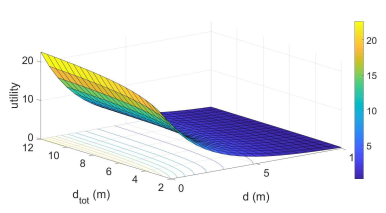
\includegraphics[width=\linewidth]{assets/3_8_b.png}
        \caption{{$\lambda=0.4$}}
        \label{fig:3.8b}
    \end{subfigure}
    \begin{subfigure}[H]{0.4\linewidth}
        \centering
        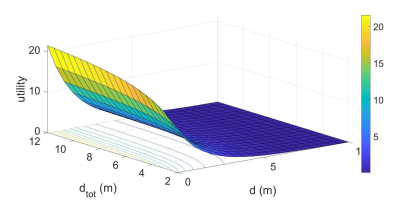
\includegraphics[width=\linewidth]{assets/3_8_c.png}
        \caption{{$\lambda=0.6$}}
        \label{fig:3.8c}
    \end{subfigure}
    \begin{subfigure}[H]{0.4\linewidth}
        \centering
        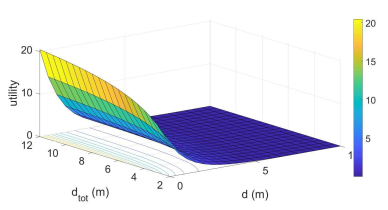
\includegraphics[width=\linewidth]{assets/3_8_d.png}
        \caption{{$\lambda=0.8$}}
        \label{fig:3.8d}
    \end{subfigure}
    \caption{{Utility function behavior: $\mathbf{I}(t_j)=25, n_c=3, d_{tot} = \sum_{k=1, k\neq i}^{n_c}(dmin(\mathbf{P}_k,\mathbf{t}_j))$. The average distance of other UAVs $d_{tot}$ has a minimum value different from zero since $n_c$ is different from zero too.}}
    \label{fig:3.8}
\end{figure}
\begin{itemize}
    \item There are no neighbors. In this case, there is one UAV in the fleet: $n_c=1$. The utility function in Eq. \ref{eq:3.3} is used.
    \item The candidate target $\mathbf{t}_j$ and the neighbors’ poses $\mathbf{P}_k$ with $k \in [1..n_c]\setminus i$ are almost confused (too close to each others). In this case $\mathbf{t}_j$ is less likely to be chosen.
\end{itemize}
Yet, this parameter $d_{tot}$ could have a high value when:
\begin{itemize}
    \item There is one UAV too far from $\mathbf{t}_j$.
    \item There are several UAVs with relatively short distance from $\mathbf{t}_j$.
\end{itemize}
So, in order to avoid these ambiguous situations, the average of $d_{tot}$ is considered by using $\frac{n_c}{d_{tot}}$.
\subsection{Goal assignment process}
In order to make appropriate UAV-to-target assignment, the utility of reaching each candidate frontier is considered. The goal assignment process is described in Algo. \ref{alg:3.5}.\\\\
For each UAV$_i$ , the utilities of reaching all the candidate targets are computed. The target $\mathbf{t}_g$ that maximizes the utility is computed and, the assignment $\theta(UAV_i,\mathbf{t}_g)$ is performed. Then, the remaining candidate targets $\mathcal{G}\setminus \mathcal{T}$ are scheduled in order to avoid to select a target too close to $\mathbf{t}_g$ , in the next iteration. Also, $\mathbf{t}_g$ is removed from $\mathcal{G}$ to prevent from assigning the same target to different robots. This assignment process is performed for the available UAVs in $\mathcal{C}$ in a sequential manner until getting all assigned targets $\mathbf{t}_g \in \mathcal{T}$ with $g \in [1..n_t]$ (See Figure \ref{fig:3.2})
\begin{algorithm}[H]
    \caption{Goal assignment algorithm.}
    \label{alg:3.5}
    \hspace*{\algorithmicindent} \textbf{Input:} {Candidate targets $\mathbf{t}_k \in \mathcal{G}, k \in [1..n_g]$ and their respective information gain $\mathbf{U}(\mathbf{t}_k)$, poses $\mathbf{P}_i$ of all robots in the considered cluster $\mathcal{C}$.}\\
    \hspace*{\algorithmicindent} \textbf{Output:} {$\theta(UAV_i,\mathbf{t}_g)$ assignment of UAV$_i$ with target $g$.}
    \begin{algorithmic}[1]
        \STATE $\mathcal{T}=\theta$
        \WHILE{no goal for UAV$_i$}
        \STATE Compute its corresponding utility of reaching each remaining candidate goal $\mathbf{U}(UAV_i,\mathbf{t}_k)$ with $\mathbf{t}_k \in \mathcal{G}\setminus \mathcal{T}$.
        \STATE $t_g=argmax_{t_k \in \mathcal{G}\setminus \mathcal{T}}(\mathbf{U}(UAV_i,\mathbf{t}_k))$.
        \STATE Schedule the information gain of the remaining candidates $\mathbf{t}_k \in \mathcal{G} \setminus \mathcal{T}$.
        \STATE $\mathcal{T}=\mathcal{T}\cup t_g$.
        \ENDWHILE
        \RETURN $\theta(UAV_i, \mathbf{t}_g)$ assignment.
    \end{algorithmic}
\end{algorithm}
\subsubsection{Stop condition}
The goal selection process is realized by each cluster/group-\textit{leader} (if $n>n-c$ ) or the Fleet- \textit{leader} (if $n=n_c$). This assignment aims to, cooperatively, distribute the robots in the environment to explore simultaneously different unknown regions. As long as candidate frontier points are still available, the \textit{leader} continues to assign targets to \textit{explorers} and they attempt to reach their assigned goals. When the \textit{leader} notices that no candidate targets are left, that means that all the environment has been explored successfully and the mission is accomplished. Thus, it has to send back to the \textit{explorers} an acknowledgment to prevent them assuming a communication loss.
\subsubsection{Loop rate}
The target assignment process is performed at each loop. The frequency of assigning targets impacts the duration and the efficiency of the mission. In a distributed approach, as soon as the UAV reaches its current target, it selects a new one without consulting the others. In a centralized approach, the first UAV to reach its current target has to wait until the others reach their respective targets. This can be a problem as soon as one of them fails or leaves the mission. Another possibility is to begin to assign targets once one UAV reaches its target. But this may generate incomplete tasks. In the proposed strategy, the frequency of assignment or loop rate $r$ is predefined depending on the average of time to reach a target (See Eq. \ref{eq:3.4}).
\begin{equation} \label{eq:3.4}
    r \in [\frac{s}{v_{i,max}},\frac{s}{v_{i,min}}]
\end{equation}
where $s$ is the maximum sensor range and $v_i$ is the UAV's velocity.
\subsubsection{Scheduling the information gain}
The information gain of each remaining candidate target $\mathbf{I}(\mathbf{t}_k)_{t-1}$ at time $t-1$ with $\mathbf{t}_k \in \mathcal{G} \setminus \{t_g\}$, that belongs to the threshold range $[r_{min} , r_{max} ]$, is scheduled at time $t$ depending on its distance w.r.t. the target $t_g$ , using Eq. \ref{eq:3.5}. Figure \ref{fig:3.9} represents an example of the function shape used to schedule the information gain. The example shows a Gaussian function with an amplitude that corresponds to the information gain maximum value; a center that corresponds to the target position $(\mathbf{t}_g(x), \mathbf{t}_g(y))$; and $\sigma_x$ and $\sigma_y$ that spread the blob in $x$ and $y$ axis, respectively.
\begin{figure}[H]
    \centering
    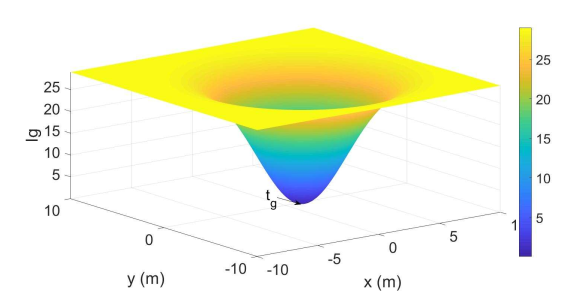
\includegraphics[scale=0.6]{assets/3_9.png}
    \caption{Example of the shape function to schedule the information gain($\mathbf{I}(\mathbf{t}_k)_{t-1}=29,(\mathbf{t}_g(x),\mathbf{t}_g(y))=(1.25,-0.275), \sigma_x=\sigma_y=3$).}
    \label{fig:3.9}
\end{figure}
\begin{equation}\label{eq:3.5}
    \mathbf{I}(\mathbf{t}_k)_t=\mathbf{I}(\mathbf{t}_k)_{t-1}(1-exp(-(\frac{(\mathbf{t}_k(x)-\mathbf{t}_g(x))^2}{2.\sigma_x^2}+\frac{(\mathbf{t}_k(y)-\mathbf{t}_g(y))^2}{2.\sigma_y^2}))),
\end{equation}
where $\mathbf{t}_k(x)$ and $\mathbf{t}_k(y)$ are the remaining candidate target coordinates; $\mathbf{t}_g(x)$ and $\mathbf{t}_g(y)$ are the target coordinates; and $\sigma_x$ and $\sigma_y$ are the spreads of the blob. The smaller the distance of the frontier point $\mathbf{t}_k$ w.r.t. the target $\mathbf{t}_g$, the smaller the information gain. When reducing the information gain, the candidate targets are less likely to be chosen and thus, robots ensure a certain distance among their future targets.
\subsection{Path planning and control}
As explained in Section 5.2 of Chapter 1, UAVs are assumed to navigate in a simplified 2D environment with a fixed $z$ value. Block \textbf{6} in Figure 1.6 is responsible for planning a path to the selected target and attempting to reach it. These tasks are ensured by the \textit{move} base\footnote{Source: \url{http://wiki.ros.org/move_base}} package.\\\\
For the navigation task, each UAV maintains a local and a global planner along with a local and a global costmap, respectively. The costmap is a 2D cell grid $\mathcal{L}$ with additional inflation that consists in propagating cost values out from occupied cells and decreasing them with distance. The global costmap has the size of the UAV’s map whereas, the local costmap has a fixed size moving window. Given a starting point – the current pose – and an endpoint – the assigned target – in the global costmap, the global planner produces a plan using a navigation function computed with Dijkstra algorithm \cite{dijkstra1959note}. It consists in following the adjacent free cells until reaching the goal. Then taking into account the local costmap, the local planner generates velocity commands for the UAV’s mobile base. A recovery rotational behavior is also performed when needed in order to clear the robot’s field of view.\\\\
The target assigned by the \textit{leader} is ensured to belong to an unknown area using the exploration strategy. The trajectory planning process is performed locally on each robot. And since the UAVs do not exchange their local maps nor fuse them, they are likely to revisit already explored areas while following the planned path. To minimize these overlapped regions during navigation, a priority is given to frontier points $\mathbf{f}_{i,j}$ to be a target for UAV$_i$ over UAV$_k$ with $k \neq i$. This helps the UAV to maintain the same direction during exploration. The \textit{move} base package is a 2D navigation stack. However, to avoid drifting on the $z$ axis, a control command is added to keep a static $z$ altitude (See Figure \ref{fig:3.10}).
\begin{figure}[H]
    \centering
    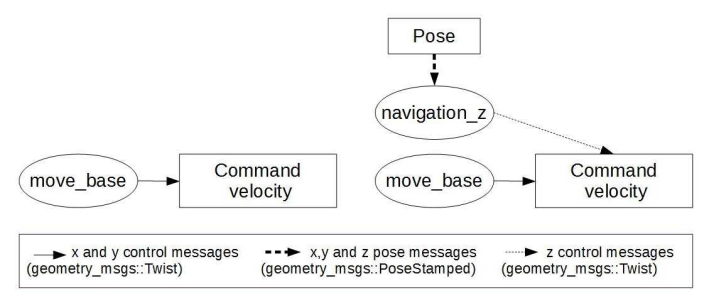
\includegraphics[scale=0.4]{assets/3_10.png}
    \caption{From 2D (left) to 3D (right) navigation stack. The \textit{navigation} z is a ROS process developed to provide a control command on the z axis.}
    \label{fig:3.10}
\end{figure}
\section{Result and discussions}
Simulations have been performed to evaluate the proposed exploration strategy. Additional tests while using relative localization have been done to measure the system performances. The simulations are performed using Robot Operating System (ROS) running on a 2.60GHz i7 Linux machine. For the quad-rotor simulation, the AR-drone model\footnote{Source: \url{http://wiki.ros.org/ardrone_autonomy}} equipped with an RGB-D camera in a forward-looking configuration, is used. A bounded unknown environment is generated using \textit{Gazebo} simulator. The number of robots used for evaluation is limited to three, however, the proposed system architecture is not constrained to a fixed number of robots.
\subsection{Parameters tuning}
For an effective evaluation of the exploration strategy, we run some tests to set the most adequate parameters configuration.
\subsubsection{Trade-off parameter $\lambda$}
The utility function (See Eq. \ref{eq:3.2}) used in the exploration strategy can be tuned, using a trade off parameter $\lambda$, between fast exploration and filling in details the map.\\\\
Figure \ref{fig:3.11} shows different runs while varying this parameter. By increasing $\lambda$, the information gained when reaching the goal is favored over the distance and thus, the cost to it, and vice versa. So, when $\lambda$ is small, the traveled distance is small and so the exploration time. Though, some times during the mission, high values of $\lambda$ are noticed to reach higher exploration rate than smaller ones.
\begin{figure}[H]
    \centering
    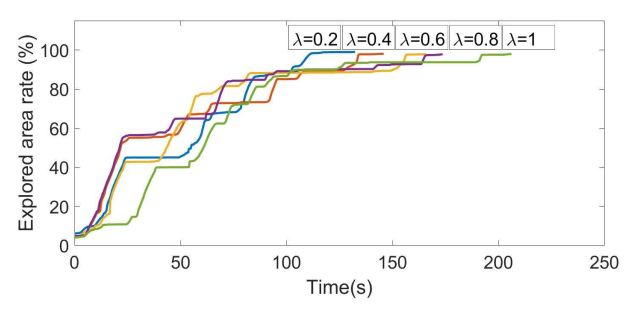
\includegraphics[scale=0.5]{assets/3_11.png}
    \caption{The impact of varying the trade off parameter $\lambda$ over exploration itme.}
    \label{fig:3.11}
\end{figure}
\subsubsection{Loop rate $r$}
The frequency or loop rate $r$ of target assignment may also affect exploration time performance. The values of $r$ vary to take into account the robot velocity $\mathbf{v}_i$ and the sensor’s maximum range $s$. The impact of varying the loop rate is evaluated in Figure \ref{fig:3.12}.
\begin{figure}[H]
    \centering
    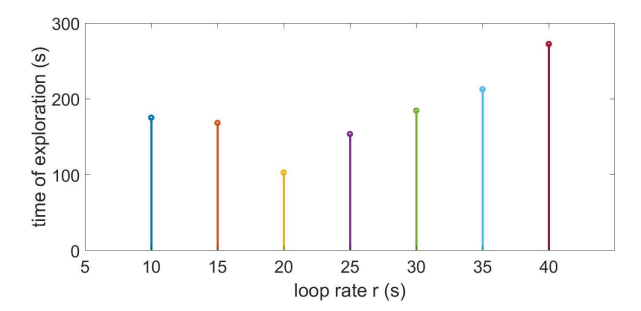
\includegraphics[scale=0.5]{assets/3_12.png}
    \caption{Exploration time while varying the loop rate $r$.}
    \label{fig:3.12}
\end{figure}
Given a robot velocity $\mathbf{v}_i=\{0.1,0.3\}m.s^{-1}$ and a maximum sensor range $s=4m$, the loop rate variates in $r \in [10,40]$. This parameter should not be too small to allow the robot to reach its target; nor too big to prevent long waiting times for the next goal assignment.
\subsubsection{Common parameters}
Depending on results in Figure \ref{fig:3.11} and Figure \ref{fig:3.12}, respectively, $\lambda$ is set to $0.2$ and $r$ to $20s$ in order to maximize the explored area rate while minimizing the mission time. The simulation parameters are summarized in Table \ref{tab:3.1}.
\begin{table}[H]
    \centering
    \caption{Common parameters.}
    \label{tab:3.1}
    \begin{tabular}{|l|l|}\hline
        \makebox[5em]{\textbf{Parameter}}                  & \makebox[5em]{\textbf{Value}}
        \\\hline
        RGB-D horizental FoV                               & $\pi/ 3$                      \\\hline
        Trade-off parameter $\lambda$                      & 0.2                           \\\hline
        RGB-D maximum range $s (m)$                        & 4                             \\\hline
        Min distance among frontiers $d (m)$               & 0.3                           \\\hline
        Occupancy grid resolution $(m)$                    & 0.05                          \\\hline
        Range to schedule the $\lg[\sigma_x,\sigma_y] (m)$ & $[3,3]$                       \\\hline
        Loop rate $l (s)$                                  & 20                            \\\hline
        Enviroment dimension $(m^2)$                       & $8 \times 8$                  \\\hline
        Linear velocity $v_i (m.s^{-1})$                   & $[0.1,0.3]$                   \\\hline
        Angular velocity $w_i (rad.s^{-1})$                & $[0.1,0.3]$                   \\\hline
    \end{tabular}
\end{table}
\subsection{Exploration strategy performances}
The proposed exploration strategy has been evaluated in terms of distribution of the robots in the environment, overlap rate, exploration time, and total traveled distance by each robot.
\subsubsection{Maps evolution during the mission}
While reaching their respective assigned goals, each robot is in charge of creating a detailed grid map of the visited area in order to get a global map of the environment. Figure \ref{fig:3.13} illustrates the growth of the reconstructed 3D occupancy grid map at different times during the mission. Note that to reach $99\%$ of coverage, a lot of time is spent.\\\\
Figure \ref{fig:3.14} shows the evolution of the respective projected 2D local grid map of two robots during a cooperative exploration mission. The global projected 2D grid map is also created and represented for evaluation (the occupancy grid matching process introduced in Algorithm 2.1 in Chapter 2 is used). The robots’ initial positions are $(1,0,0)$ for UAV$_1$ and $(1,-3,0)$ for UAV$_2$. Despite a relatively close initial position, the proposed strategy effectively spreads the robots so that UAV$_1$ is in charge of the left side of the environment and UAV$_2$ of the right one.
\subsubsection{Frontier points evolution during the mission}
The target is chosen from the candidate frontier points that define the edges of an environment not previously explored. These candidates are selected from the final frontier points of each UAV in the fleet (See Figure \ref{fig:3.15}). During the exploration mission, the local map size increases, which leads to an increasing number of local frontier points. At the beginning of the exploration, the number of candidate frontier points increases, but as soon as the exploration evolves in time, their number decreases. At the end of the mission, when all the environment is explored, no candidate frontier points should be left.
\subsubsection{UAV's trajectories during the mission}
Figure \ref{fig:3.16} shows the explored map with the trajectories using one, two and three UAVs. The UAVs try to explore the full environment while avoiding already explored areas. In a cooperative way, each UAV is in charge of visiting an area by reaching a target that belongs to a non-explored environment. These targets are assigned by the \textit{Leader} which, even if the initial poses of the UAVs are relatively close, effectively spreads them into unknown areas. The global map is composed of the superposition of all UAVs’ local maps.
\begin{figure}[H]
    \centering
    \begin{subfigure}[H]{0.3\linewidth}
        \centering
        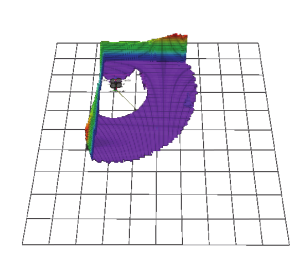
\includegraphics[width=\linewidth]{assets/3_13_a.png}
        \caption{{$3\%$ rate $(5s).$}}
        \label{fig:3.13a}
    \end{subfigure}
    \begin{subfigure}[H]{0.3\linewidth}
        \centering
        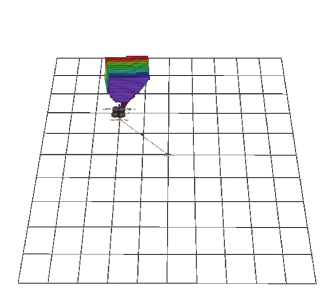
\includegraphics[width=\linewidth]{assets/3_13_b.png}
        \caption{{$20\%$ rate $(28s).$}}
        \label{fig:3.13b}
    \end{subfigure}
    \begin{subfigure}[H]{0.3\linewidth}
        \centering
        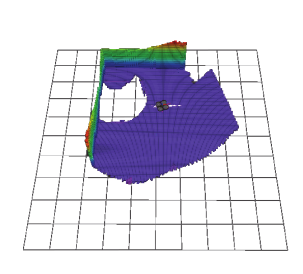
\includegraphics[width=\linewidth]{assets/3_13_c.png}
        \caption{{$31\%$ rate $(50s).$}}
        \label{fig:3.13c}
    \end{subfigure}
    \begin{subfigure}[H]{0.3\linewidth}
        \centering
        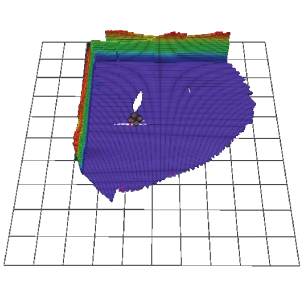
\includegraphics[width=\linewidth]{assets/3_13_d.png}
        \caption{{$40\%$ rate $(69s).$}}
        \label{fig:3.13d}
    \end{subfigure}
    \begin{subfigure}[H]{0.3\linewidth}
        \centering
        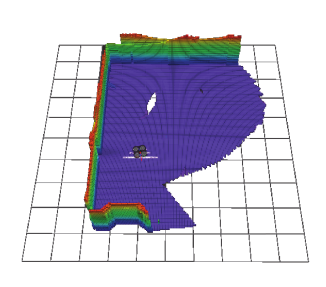
\includegraphics[width=\linewidth]{assets/3_13_e.png}
        \caption{{$50\%$ rate $(75s).$}}
        \label{fig:3.13e}
    \end{subfigure}
    \begin{subfigure}[H]{0.3\linewidth}
        \centering
        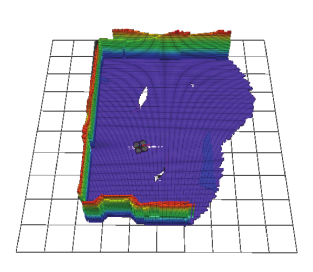
\includegraphics[width=\linewidth]{assets/3_13_f.png}
        \caption{{$60\%$ rate $(83s).$}}
        \label{fig:3.13f}
    \end{subfigure}
    \begin{subfigure}[H]{0.3\linewidth}
        \centering
        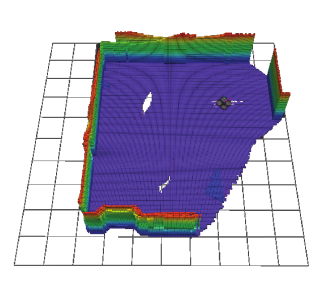
\includegraphics[width=\linewidth]{assets/3_13_g.png}
        \caption{{$70\%$ rate $(98s).$}}
        \label{fig:3.13g}
    \end{subfigure}
    \begin{subfigure}[H]{0.3\linewidth}
        \centering
        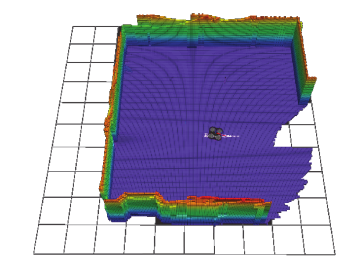
\includegraphics[width=\linewidth]{assets/3_13_h.png}
        \caption{{$81\%$ rate $(127s).$}}
        \label{fig:3.13h}
    \end{subfigure}
    \begin{subfigure}[H]{0.3\linewidth}
        \centering
        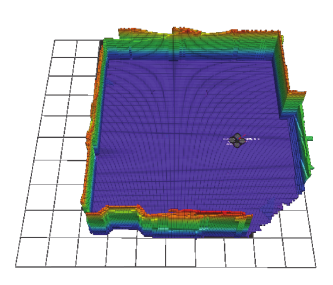
\includegraphics[width=\linewidth]{assets/3_13_i.png}
        \caption{{$90\%$ rate $(133s).$}}
        \label{fig:3.13i}
    \end{subfigure}
    \begin{subfigure}[H]{0.3\linewidth}
        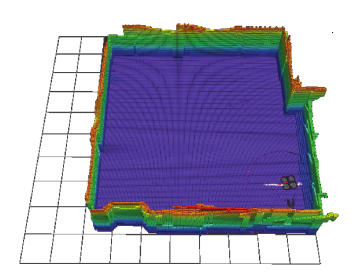
\includegraphics[width=\linewidth]{assets/3_13_j.png}
        \caption{{$99\%$ rate $(202s).$}}
        \label{fig:3.13j}
    \end{subfigure}
    \caption{Ratio of explored space during time for one UAV.}
    \label{fig:3.13}
\end{figure}
\begin{figure}[H]
    \centering
    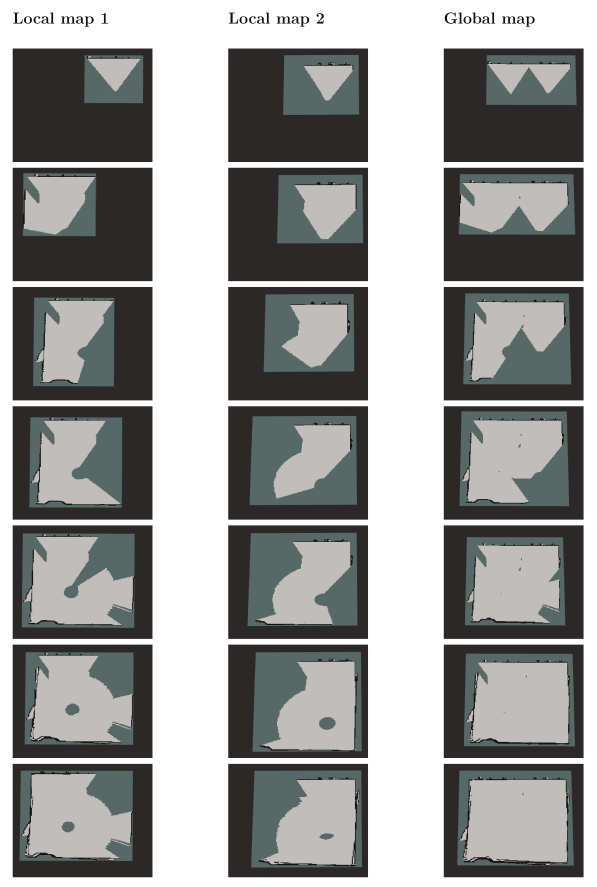
\includegraphics[scale=0.5]{assets/3_14.png}
    \caption{Coordinated exploration using two robots. Columns 1, 2 and 3 show the evolution of the local map of the UAV$_1$, the UAV$_2$ and the global map over time, respectively.}
    \label{fig:3.14}
\end{figure}
\begin{figure}[H]
    \centering
    \begin{subfigure}[H]{0.7\linewidth}
        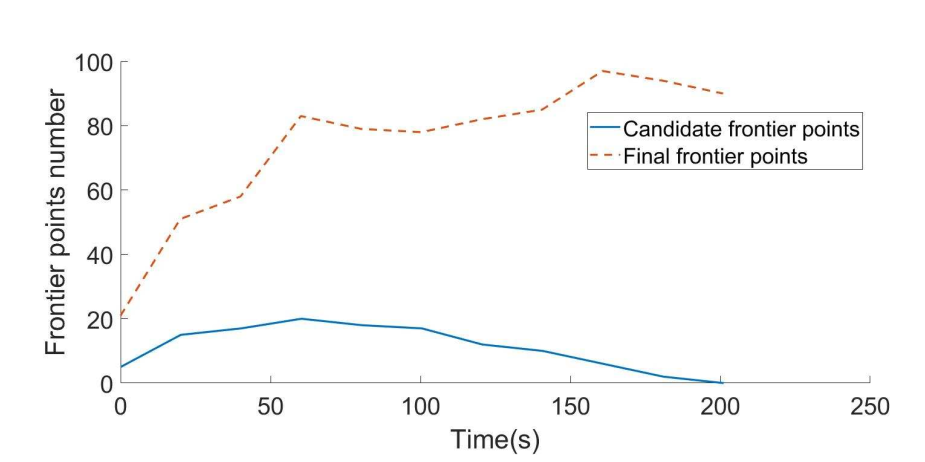
\includegraphics[width=\linewidth]{assets/3_15_a.png}
        \caption{{One UAV.}}
        \label{fig:3.15a}
    \end{subfigure}
    \begin{subfigure}[H]{0.7\linewidth}
        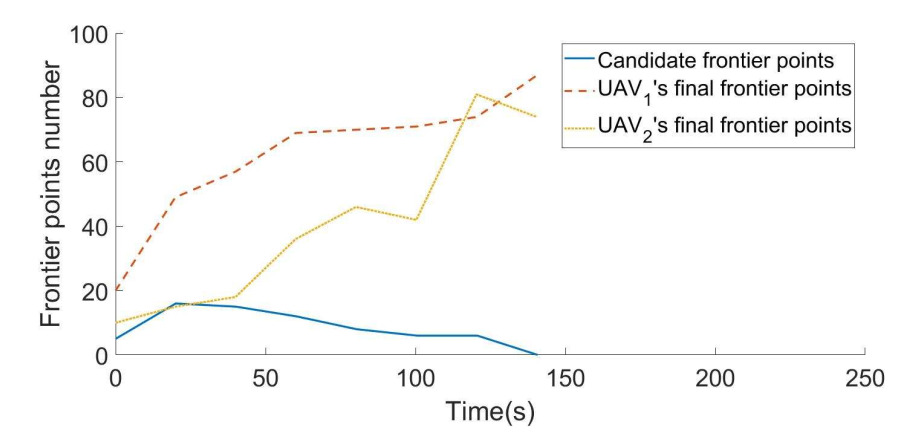
\includegraphics[width=\linewidth]{assets/3_15_b.png}
        \caption{{Two cooperative UAVs.}}
        \label{fig:3.15b}
    \end{subfigure}
    \begin{subfigure}[H]{0.7\linewidth}
        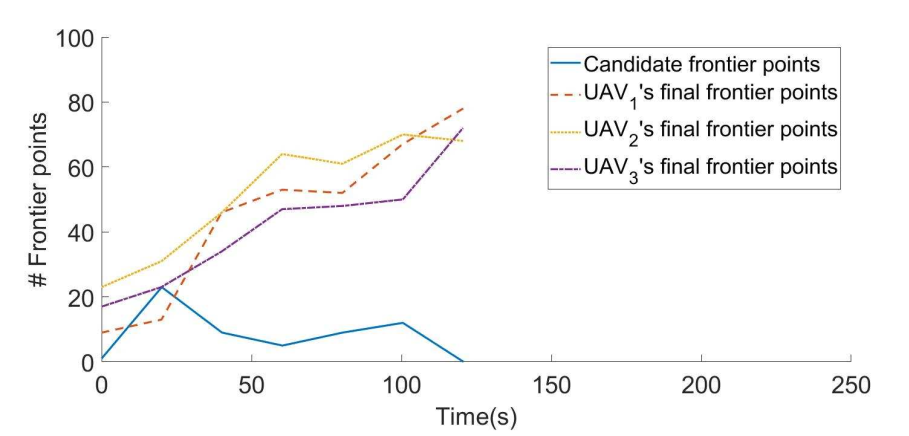
\includegraphics[width=\linewidth]{assets/3_15_c.png}
        \caption{{Three cooperative UAVs}}
        \label{fig:3.15c}
    \end{subfigure}
    \caption{The evolution of candidate and final frontier points numbers during cooperative exploration.}
    \label{fig:3.15}
\end{figure}
\begin{figure}[H]
    \centering
    \begin{subfigure}[H]{0.5\linewidth}
        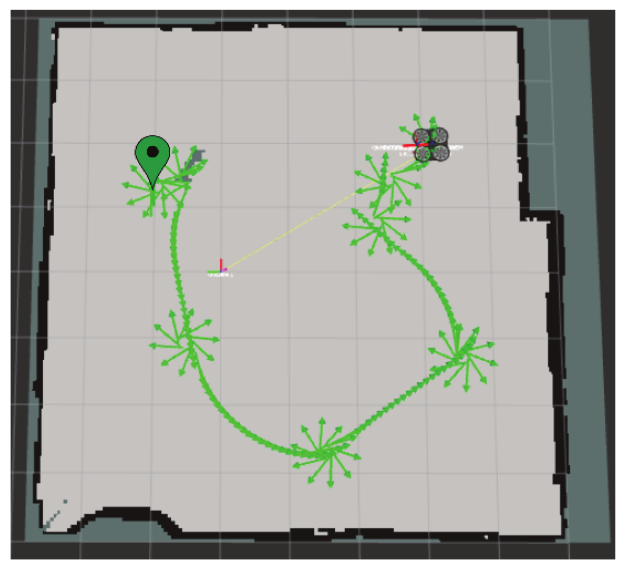
\includegraphics[width=\linewidth]{assets/3_16_a.png}
        \caption{{One UAV.}}
        \label{fig:3.16a}
    \end{subfigure}
    \begin{subfigure}[H]{0.5\linewidth}
        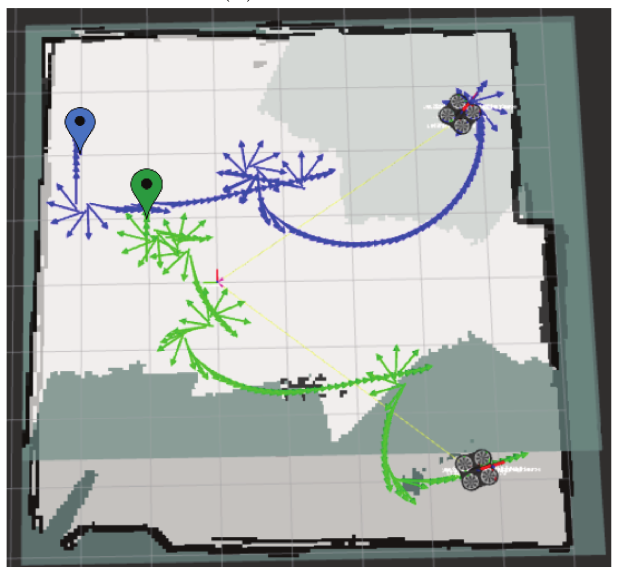
\includegraphics[width=\linewidth]{assets/3_16_b.png}
        \caption{{Two cooperative UAVs.}}
        \label{fig:3.16b}
    \end{subfigure}
    \begin{subfigure}[H]{0.5\linewidth}
        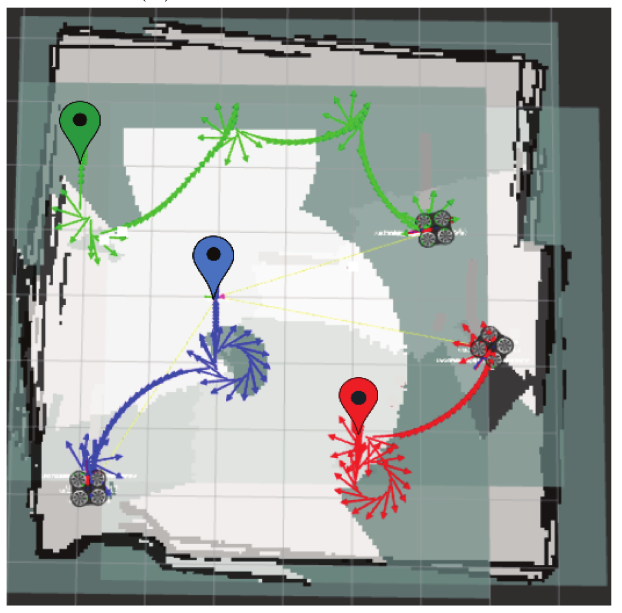
\includegraphics[width=\linewidth]{assets/3_16_c.png}
        \caption{{Three cooperative UAVs}}
        \label{fig:3.16c}
    \end{subfigure}
    \caption{Projected 2D map in a coordinated exploration with a team of one, two and three UAVs. Green, blue and red markers and arrows define, respectively, the initial position and the trajectory of UAV1, UAV2 and UAV3.}
    \label{fig:3.16}
\end{figure}
\subsubsection{Goal assignment evaluation: Distribution of the robots in the environment}
The goal assignment process is performed according to the algorithm described in Section 3.6. Nevertheless, after assigning a target to the first robot in the list, the same target or another one close to it may be assigned to the second robot in the list. To overcome these issues, the information gains of the remaining candidate targets are scheduled. This allows to discard an already assigned target and keep a certain distance between the new target and the previous one assigned.\\\\
Suppose that a target is assigned to the first robot in the cluster list. Figure \ref{fig:3.17} shows the goal selected for the second robot when a sequential assignment is performed:
\begin{itemize}
    \item Without further frontier points processing (See Figure \ref{fig:3.17b}). Consequently, the same target is assigned to two different robots.
    \item While removing the assigned target from the remaining candidate frontier points (See Figure \ref{fig:3.17c}). Consequently, the second target is relatively close to the first one assigned.
    \item While scheduling the information gain after each target assignment (See Figure \ref{fig:3.17d}). Consequently, the assigned targets are spaced out into the environment. The information gain is scheduled following Eq. \ref{eq:3.5}. The information gain value increases with distance to the candidate target $\mathbf{t}_g$.
\end{itemize}
The goal assignment process may sometimes be not optimal since it depends on the robots’ order in the list. For example, suppose that robots UAV$_i$ and UAV$_j$ have the same best target assignment t k such that it offers the maximum utility over candidate frontier points where Eq.\ref{eq:3.6} and Eq. \ref{eq:3.7} are verified.
\begin{equation}\label{eq:3.6}
    \mathbf{t}_k=argmax_{t_m}\mathbf{U}(UAV_i,\mathbf{t}_m)
\end{equation}
with $\mathbf{t}_m \in \mathcal{G}$.
\begin{equation}\label{eq:3.7}
    \mathbf{t}_k=argmax_{t_n}\mathbf{U}(UAV_j, \mathbf{t}_n)
\end{equation}
with $\mathbf{t}_n \in \mathcal{G}$.\\
UAV$_i$ have another candidate frontier point $\mathbf{t}_l$ with:
\begin{equation}\label{eq:3.8}
    \mathbf{\mathit{U}}(UAV_i, \mathbf{t}_k) > \mathbf{\mathit{U}}(UAV_i,\mathbf{t}_l) > \mathbf{\mathit{U}}(UAV_j, \mathbf{t}_k)
\end{equation}

\begin{figure}[H]
    \centering
    \begin{subfigure}[H]{0.6\linewidth}
        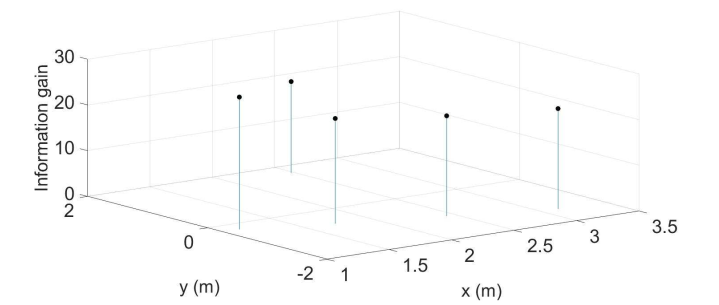
\includegraphics[width=\linewidth]{assets/3_17_a.png}
        \caption{{Candidate targets.}}
        \label{fig:3.17a}
    \end{subfigure}
    \begin{subfigure}[H]{0.6\linewidth}
        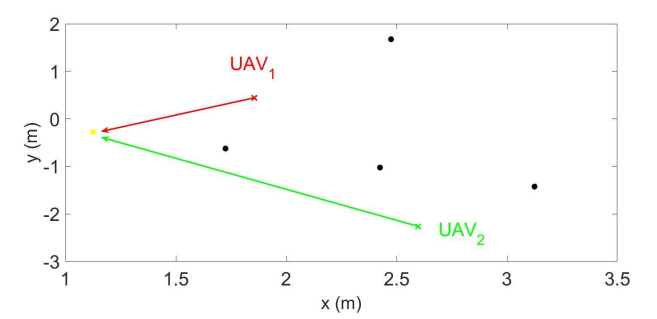
\includegraphics[width=\linewidth]{assets/3_17_b.png}
        \caption{{Case 1.}}
        \label{fig:3.17b}
    \end{subfigure}
    \begin{subfigure}[H]{0.6\linewidth}
        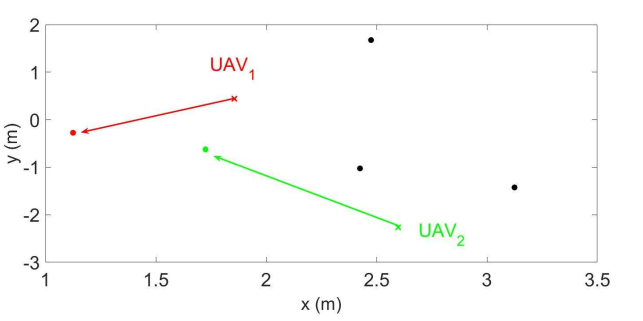
\includegraphics[width=\linewidth]{assets/3_17_c.png}
        \caption{{Case 2.}}
        \label{fig:3.17c}
    \end{subfigure}
    \begin{subfigure}[H]{0.6\linewidth}
        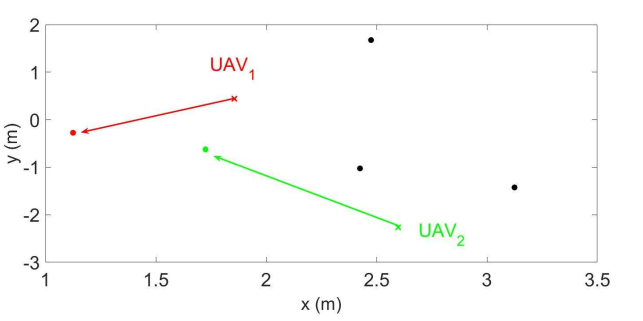
\includegraphics[width=\linewidth]{assets/3_17_c.png}
        \caption{{Case 3.}}
        \label{fig:3.17d}
    \end{subfigure}
    \caption{Goal assignment: After assigning a target to UAV$_1$ , a target is assigned in a sequential manner to UAV$_2$ . (a) represents the candidate frontier points with their respective information gain. (b), (c), and (d) represent, respectively, the targets assignment when: No further process is performed for the remaining candidate targets; UAV$_1$ ’s target is removed from the remaining candidate targets and; the information gain of the remained candidate targets are scheduled.}
    \label{fig:3.17}
\end{figure}
So the optimal solution would be to assign $\mathbf{t}_l$ to UAV$_i$ and $\mathbf{t}_k$ to UAV$_j$ . But, if UAV$_i$ is the first in the list, $\mathbf{t}_k$ is assigned to it and another candidate frontier point with less utility than $\mathbf{t}_k$, is assigned to UAV$_j$. Thus, the solution with sequential goal assignment is not always optimal.\\\\
To overcome this problem, all the numbers of possible combination $\frac{n_g!}{n_g!(n_g-n_c)!}$ with $n_g$ the number of candidate targets and $n_c$ the number of robots, need to be considered. This increases considerably the computation time by increasing the number of robots. Therefore, in the proposed algorithm, sequential assignment is favored over computing all possible permutations.
\subsubsection{Explored space rate evaluation}
This evaluation aims at quantifying the amount of explored spaces during the mission. Figure \ref{fig:3.18} shows the explored space rate performed by each UAV in the fleet. The more UAVs in the environment, the less the exploration rate demanded by each one. A robot has no need to continue exploring an area if it has already been explored by another one. Thus, the mission time is considerably reduced.
\subsubsection{Overlap rate evaluation}
The use of an effective goal assignment process should limit the generated overlap. In Figure \ref{fig:3.19}, the time evolution of overlap is evaluated using two cooperative robots. The overlap undergoes a significant increase at the end of the exploration to reach $33\%$. This is explained by the closeness of the local maps at the end of the mission to precisely fill the global grid map.
\begin{figure}[H]
    \centering
    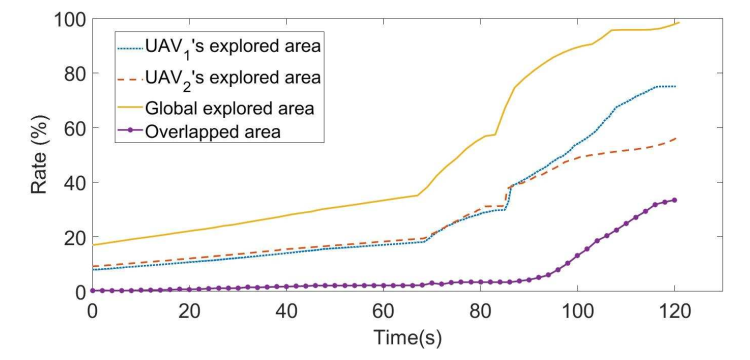
\includegraphics[scale=0.4]{assets/3_19.png}
    \caption{Explored and overlapped area rate using two cooperative UAVs.}
    \label{fig:3.19}
\end{figure}
\subsubsection{Traveled distance evaluation}
To effectively evaluate the exploration strategy performance in terms of distance traveled by each UAV, different runs with one, two and three UAVs have been conducted where explored area rate reaches almost $99\%$. Figure \ref{fig:3.20} shows the distance traveled by each UAV in the fleet during the mission.
\begin{figure}[H]
    \centering
    \begin{subfigure}[H]{0.7\linewidth}
        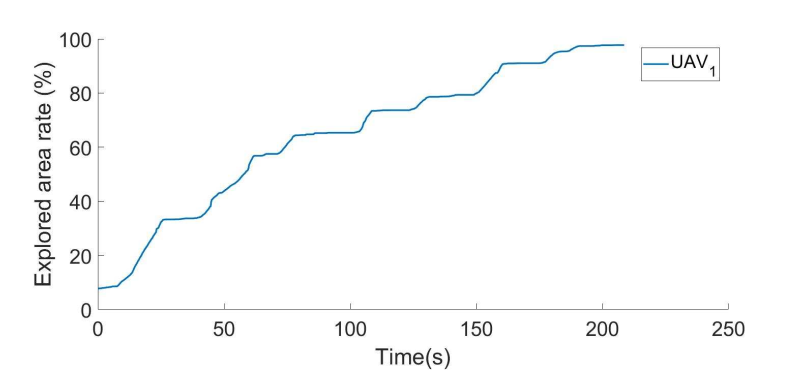
\includegraphics[width=\linewidth]{assets/3_18_a.png}
        \caption{{One UAV.}}
        \label{fig:3.18a}
    \end{subfigure}
    \begin{subfigure}[H]{0.7\linewidth}
        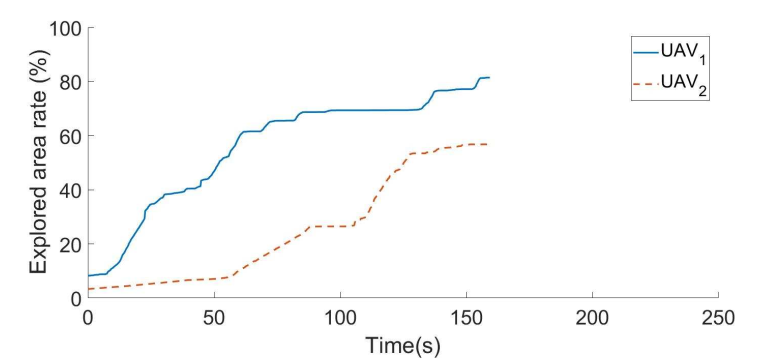
\includegraphics[width=\linewidth]{assets/3_18_b.png}
        \caption{{Two cooperative UAVs.}}
        \label{fig:3.18b}
    \end{subfigure}
    \begin{subfigure}[H]{0.7\linewidth}
        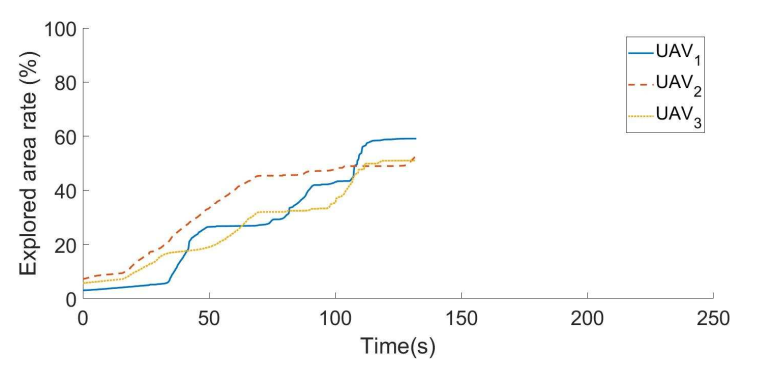
\includegraphics[width=\linewidth]{assets/3_18_c.png}
        \caption{{Three cooperative UAVs}}
        \label{fig:3.18c}
    \end{subfigure}
    \caption{Explored space rate with one, two and three UAVs.}
    \label{fig:3.18}
\end{figure}
\begin{figure}[H]
    \centering
    \begin{subfigure}[H]{0.7\linewidth}
        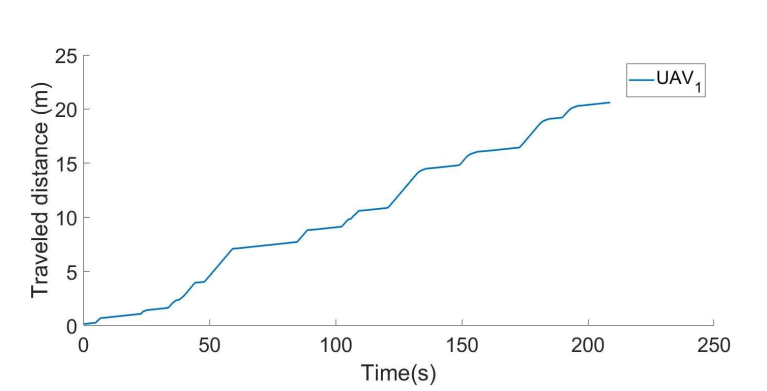
\includegraphics[width=\linewidth]{assets/3_20_a.png}
        \caption{{One UAV.}}
        \label{fig:3.20a}
    \end{subfigure}
    \begin{subfigure}[H]{0.7\linewidth}
        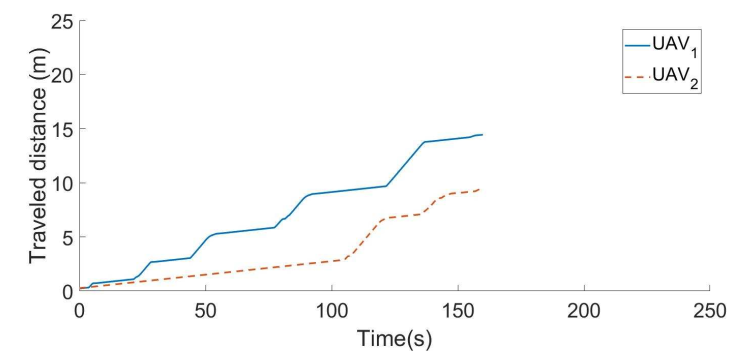
\includegraphics[width=\linewidth]{assets/3_20_b.png}
        \caption{{Two cooperative UAVs.}}
        \label{fig:3.20b}
    \end{subfigure}
    \begin{subfigure}[H]{0.7\linewidth}
        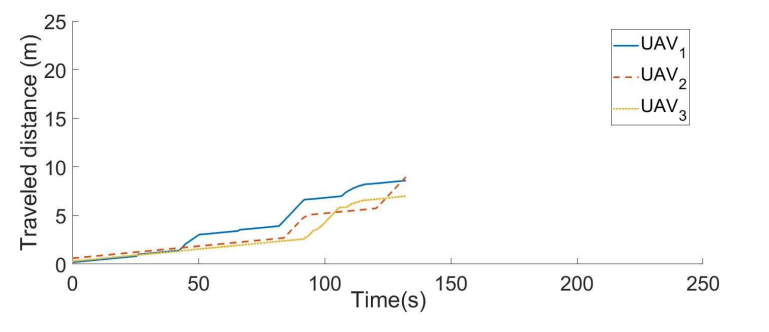
\includegraphics[width=\linewidth]{assets/3_20_c.png}
        \caption{{Three cooperative UAVs}}
        \label{fig:3.20c}
    \end{subfigure}
    \caption{Traveled distance by each UAV with one, two and three cooperative UAVs.}
    \label{fig:3.20}
\end{figure}
The distances traveled by each UAV using one, two and three UAVs in the fleet are compared in Figure \ref{fig:3.21}. This distance decreases with the number of UAVs. The average distance traveled by each UAV is reduced by $55\%$ for 2 UAVs and by $62\%$ for 3 UAVs. The error of the traveled distance is slightly reduced from one to two and three UAVs.
\begin{figure}[H]
    \centering
    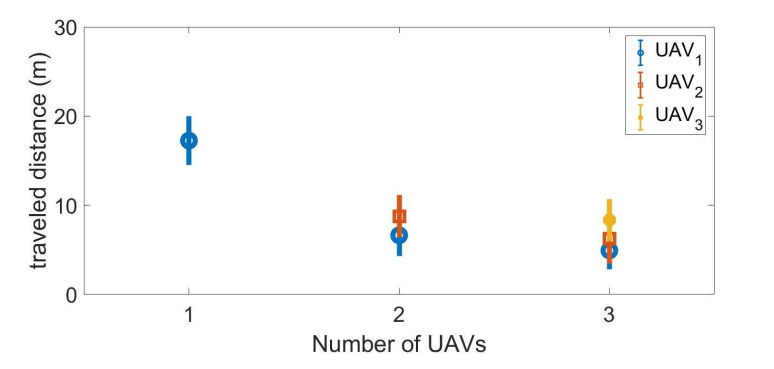
\includegraphics[scale=0.4]{assets/3_21.png}
    \caption{Traveled distance evaluation.}
    \label{fig:3.21}
\end{figure}
\subsubsection{Exploration time evaluation}
For the exploration time evaluation, different runs have been performed using 1, 2 and 3 UAVs. Figure \ref{fig:3.22} shows that the average of exploration time decreases when the number of robots in the fleet increases. The computed error decreases as well. The time is reduced by $25\%$ for 2 UAVs and by $30\%$ for 3 UAVs. The exploration time and distance are not divided by 2 or 3 when multiplying by 2 or 3 the number of robots, respectively. During these simulations, the robots’ initial positions are: $(1,0,0)$ for one UAV; $(1,0,0)$ and $(1,-3,0)$ for two UAVs; and $(1,1,0)$, $(1,-1,0)$ and $(1,-3,0)$ for three UAVs.
\begin{figure}[H]
    \centering
    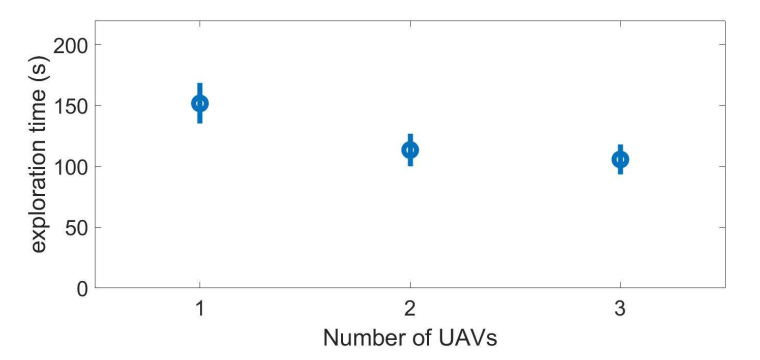
\includegraphics[scale=0.4]{assets/3_22.png}
    \caption{Average exploration time.}
    \label{fig:3.22}
\end{figure}
The results presented in Section 4.2 were evaluated without a relative localization. So, for a more challenging realistic scenario, runs with relative localization algorithm have been performed to evaluate system performances using SLAM.
\subsection{Exploration mission using relative localization algorithm}
Toward a more realistic scenario, the ORB-SLAM2 approach (introduced in Section 5 of Chapter 2) has been implemented to perform relative localization (See Figure \ref{fig:3.23}).
\begin{figure}[H]
    \centering
    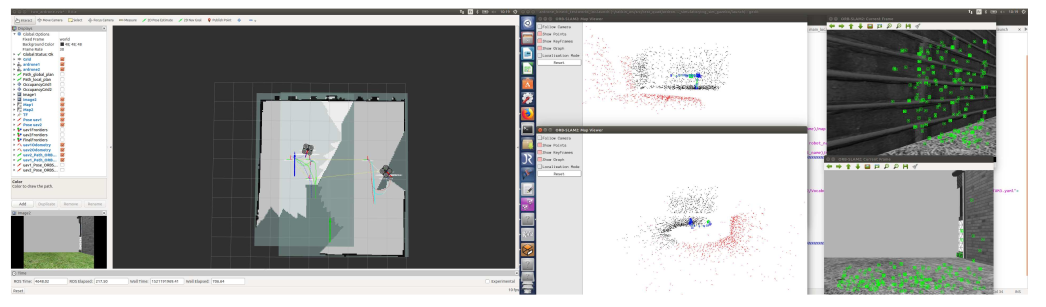
\includegraphics[scale=0.3]{assets/3_23.png}
    \caption{Two UAVs navigation using ORB-SLAM2. Rviz image (left) shows, for each UAV, the constructed 2D occupancy grid map, its estimated trajectory and the corresponding ground truth. The point cloud (middle) represent the sparse reconstruction of the environment made by each UAV. And, the green markers (right) represent the features computed by each UAV to perform localization.}
    \label{fig:3.23}
\end{figure}
Each robot performs SLAM where it constructs its map in its local reference frame $^WF_i$ , and estimates its relative pose $\mathbf{p}_i$ within it. Then, the fleet performs cooperative explo- ration using some specific information exchanged among UAVs. But, these information have to be in a common reference frame. Therefore, information such as the pose $\mathbf{p}_i$ and the frontier points $\mathbf{f}_{i,j}$ are necessarily transformed into the global reference frame $^0W$ before being exchanged. Hence, the \textit{leader} makes all the needed computation and sends back to the \textit{explorers} the targets in $^0W$. When a robot receives its assigned goal, it transforms it into $^WF_i$ to plan a path to it.\\\\
To perform a transformation from local reference $^WF_i$ to global one $^0W$, the robot has to know – at least – its initial pose w.r.t. $^0W$. As explained in Section 5.2 of Chapter 1, the global reference frame of the environment is initialized such that it coincides with the local reference frame of the first group-\textit{leader} in the fleet which is UAV$_1$ in the considered example of Equation \ref{eq:3.9}.
\begin{equation}\label{eq:3.9}
    ^0W\equiv ^WF_1,
\end{equation}
Then, by detecting this robot using tags mounted on it, the other robots are able to estimate their respective transform to it $^{F_j}\begin{bmatrix}\mathbf{R} & \mathbf{t}\end{bmatrix}_{F_1}, j \in [2..n_c]$. For simulation evaluations, the information of transform – computed while detecting the tag – are assumed to be known. Figure \ref{fig:3.24} shows the exploration rate evolution during the exploration mission while using ORB-SLAM2 as the relative localization approach. The mission time using ORB-SLAM2 is reduced by $43\%$ for 2 UAVs instead of 1 UAV.
\begin{figure}[H]
    \centering
    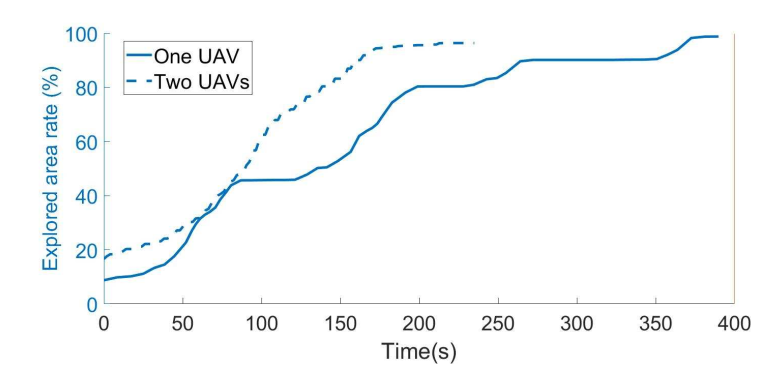
\includegraphics[scale=0.4]{assets/3_24.png}
    \caption{Explored area rate evolution during exploration mission with one and two UAVs while performing ORB-SLAM2 by each UAV.}
    \label{fig:3.24}
\end{figure}
The exploration time when using a relative localization (See Figure \ref{fig:3.24}) is relatively important compared to the exploration without SLAM (See Figure \ref{fig:3.18}) since the velocity has been considerably reduced.
\section{Conclusion}
In this chapter, we presented a state of the art of multi-robot exploration mission including the strategy used to assign a robot to a target and an utility function adopted to estimate the interest of reaching it. Then, we introduced an exploration strategy based on the group-\textit{leader} decision making. The robot-to-target assignment is performed using a novel utility function. This function makes a trade-off between fast exploration and getting a detailed grid map, and also takes into account the distance of each robot in the group from the unexplored set of targets. Also, we propose to schedule the information gain in order to efficiently spread the UAVs into the environment. Moreover, the strategy adopted exchanges the frontier points instead of a whole copy of the local map.\\\\
Results show that the proposed cooperative exploration strategy minimizes the global exploration time by $25\%$ for 2 UAVs and by $30\%$ for 3 UAVs, while minimizing the average traveled distance by each UAV by $55\%$ for 2 UAVs and by $62\%$ for 3 UAVs. Furthermore, the strategy was evaluated using a relative localization algorithm where the exploration time was reduced by $43\%$ for 2 UAVs instead of 1 UAV.
%------------------CHAPTER 4------------------------------------------------%
\chapter{Giao tiếp giữa các robot}
\section{Giới thiệu}
Một chủ đề quan trọng trong các hệ thống nhiều robot là giao tiếp giữa các robot. Tính năng này được sử dụng để điều phối và chia sẻ thông tin cụ thể. Một đội có thể được triển khai trong một số nhiệm vụ trong các khu vực tương đối khác biệt và thù địch. Tuy nhiên, những môi trường này có thể không có cơ sở hạ tầng mạng sẵn có, ngoài các liên kết truyền thông không lý tưởng.\\\\
% This chapter highlights one of the most challenging points in MRS, which is the inter- robot communication. This problem can be addressed from different perspectives; but, we have chosen to study two sub-problems, which are: network typology, and network topology and strategy for MRS robustness.
Chương này nhấn mạnh một trong những điểm thách thức nhất trong MRS, đó là giao tiếp giữa các robot. Vấn đề này có thể được giải quyết từ các quan điểm khác nhau; nhưng, chúng tôi đã lựa chọn nghiên cứu hai vấn đề nhỏ, đó là: định dạng mạng, cấu trúc liên kết mạng và chiến lược cho sự mạnh mẽ của MRS.
\section{Phân loại mạng}
% The network is used to link between different entities and to establish possible communi- cation between them. Several network types exist and can be classified in different ways.
Mạng được sử dụng để liên kết giữa các thực thể khác nhau và để thiết lập giao tiếp có thể có giữa chúng. Một số loại mạng tồn tại và có thể được phân loại theo nhiều cách khác nhau.
\subsection{Chế độ cơ sở hạ tầng so với chế độ không có cơ sở hạ tầng}
Để quản lý cơ sở hạ tầng mạng, các chế độ hiện có có thể được phân loại thành hai loại chính \cite{bekmezci2013flying},\cite{hayat2015experimental}. Loại đầu tiên là chế độ cơ sở hạ tầng, có thể được gọi là chế độ Điểm truy cập (AP) và loại thứ hai là chế độ không có cơ sở hạ tầng, gọi là Ad Hoc mode (Xem Hình \ref{fig:4.1}). Trong chế độ AP, giao tiếp UAV-to-UAV được thực hiện thông qua cơ sở hạ tầng (AP, bộ định tuyến, v.v.), không giống như chế độ Ad Hoc trong đó các nút giao tiếp trực tiếp với nhau. Chế độ Ad Hoc còn được gọi là chế độ ngang hàng. Mạng Ad Hoc có thể phát triển thành một chế độ ngang hàng khác được gọi là mạng lưới bằng cách cho phép khả năng đa bước. Thật vậy, mạng Ad-Hoc không có bất kỳ khả năng cố hữu nào cho đa bước. Các nút giao tiếp với nhau khi chúng nằm trong phạm vi giao tiếp của nhau. Trong khi đó, trong mạng lưới, các nút có thể giao tiếp trực tiếp hoặc thông qua một hoặc nhiều nút trung gian.
\begin{figure}[H]
    \centering
    \includegraphics[scale=0.4]{assets/4_1.png}
    \caption{Chế độ hạ tầng (trái) và chế độ không có hạ tầng (phải).}
    \label{fig:4.1}
\end{figure}
\begin{table}[H]
    \centering
    \caption{Chế độ cơ sở hạ tầng so với chế độ không có cơ sở hạ tầng.}
    \label{tab:4.1}
    \begin{tabular}{|l|p{4.5cm}|p{4.5cm}|}\hline
                            & \textbf{Chế độ cơ sở hạ tầng}                 & \textbf{Chế độ không có cơ sở hạ tầng}
        \\\hline
        \textbf{Ưu điểm}    & Giao tiếp đáng tin cậy                        & Kết nối trực tiếp với nhau, dễ thiết lập, mạnh mẽ với lỗi nút, cho phép mở rộng và điều chỉnh trong cấu trúc liên kết mạng. \\\hline
        \textbf{Nhược điểm} & Phần cứng đắt, phức tạp, phạm vị bị hạn chế . & Thừa trong kết nối mạng, khó bảo trì.                                                                                       \\\hline
        \textbf{Tiêu chuẩn} & 802.11                                        & 802.11, 802.15, 802.16                                                                                                      \\\hline
    \end{tabular}
\end{table}
Ban đầu, robot phải thực hiện nhiệm vụ của chúng trong môi trường không có cơ sở hạ tầng mạng. Trên thực tế, chúng trao đổi thông tin khi chúng hoạt động như một bộ định tuyến và như một AP. Vì vậy, hệ thống MRS có thể được xem như một mạng Ad Hoc di động theo quan điểm giao tiếp.
\subsection{Phân loại mạng Ad Hoc}
Mạng Ad Hoc là mạng được sử dụng phổ biến để quản lý giao tiếp đa robot. Với mạng này, mỗi robot có thể di chuyển tự do và chuyển tiếp các gói tin đến và từ mỗi robot khác tùy thuộc vào phương thức phân phối dữ liệu \cite{bouachir2014conception}. Mạng này được đặc trưng bởi chất lượng dịch vụ phức tạp, trong đó giao thức định tuyến xác định đường đi tối ưu của thông tin có tính đến sự thay đổi thường xuyên của cấu trúc liên kết. Thêm vào đó, sẽ rẻ hơn nếu nhận ra loại mạng này thay vì các loại khác (vệ tinh, di động, v.v.).\\\\
Mạng Ad Hoc có thể được phân loại thành ba loại chính là Mobile Ah doc NETwork (MANET), Vehicle Ah doc NETwork (VANET) và Flying Ad hoc NETworks (FANET). Nói chung, đối với hệ thống đa UAV, mô hình FANET được sử dụng. Bảng \ref{tab:4.2} mô tả chi tiết mỗi đặc điểm của danh mục \cite{bekmezci2013flying}, \cite{maistrenko2016experimental}, phân tích dự đoán của chúng tôi.
\begin{table}[H]
    \centering
    \caption{So sánh giữa MANET, VANET, FANET và mô hình mạng của chúng tôi.}
    \label{tab:4.2}
    \begin{tabular}{|p{2.8cm}|p{1.5cm}|p{1.5cm}|p{1.8cm}|p{1.8cm}|}\hline
        \textbf{Đặc điểm}                                                 & \textbf{MANET}                                      & \textbf{VANET}                       & \textbf{FANET}                                                                                 & \textbf{Mô hình mạng của chúng tôi}
        \\\hline
        \textbf{Tính di động}                                             & Người ở một số địa hình nhất định                   & Phương tiện ở cao tốc                & Máy bay trong kế hoạch 3D                                                                      & 3D                                  \\\hline
        \textbf{Mức độ di động}                                           & $+$                                                 & $+$                                  & $++$                                                                                           & $++$                                \\\hline
        \textbf{Chế độ di động}                                           & Điểm cách ngẫu nhiên với hướng và tốc độ ngẫu nhiên & Có khả năng dự đoán cao trên đường   & Không được xác định trước (mô hình chuyển động ngẫu nhiên của UAV, mô hình dựa trên pheromone) & Có thể dự đoán                      \\\hline
        \textbf{Thay đổi cấu trúc liên kết}                               & $+$                                                 & $+$                                  & $++$                                                                                           & $++$                                \\\hline
        \textbf{Khoảng cách giữa các nút}                                 & $+$                                                 & $+$                                  & $++$                                                                                           & $+$                                 \\\hline
        \textbf{Mật độ nút}                                               & $++$                                                & $++$                                 & $+$                                                                                            & $+$                                 \\\hline
        \textbf{Mô hình truyền thanh}                                     & Sự hiện diện hiếm hoi của đường ngắm                & Sự hiện diện hiếm hoi của đường ngắm & Sự hiện diện thường xuyên của đường ngắm                                                       & Luôn có mặt của đường ngắm          \\\hline
        \textbf{Công suất tiêu thụ và công suất tính toán thời gian sống} & $+$                                                 & $+$                                  & $++$                                                                                           & $++$                                \\\hline
        \textbf{Tiêu chuẩn}                                               & IEEE 802.11, 802.15, 802.15.4, 802.16 and 802.20    & IEEE 802.11p                         & IEEE 802.11                                                                                    & ?                                   \\\hline
    \end{tabular}
\end{table}
So sánh cho thấy FANET là mạng gần nhất với kỳ vọng của mô hình của chúng tôi. Do đó, trong số các tiêu chuẩn hiện có cho loại mạng này, IEEE 802.11b và IEEE 802.11g cung cấp tốc độ dữ liệu cao và thường được sử dụng cho các hệ thống nhiều robot.
\subsection{Phân loại cấu trúc liên kết mạng}
Cấu trúc liên kết mạng xác định điểm đầu, điểm cuối và đường dẫn của thông tin trong mạng. Đã cho các điểm mục tiêu, cấu trúc liên kết xác định tất cả các con đường có thể để đạt được chúng.\\\\
Từ quan điểm phần mềm, mạng chủ yếu có thể được phân loại theo ba cấu trúc liên kết (Xem Hình \ref{fig:4.2}\footnote{Source: From user 1983 on Wikipedia. Licensed CC BY-SA}):
\begin{figure}[H]
    \centering
    \includegraphics[scale=0.4]{assets/4_2.png}
    \caption{Mạng tập trung (trái), phi tập trung (giữa) và mạng phân tán (phải).}
    \label{fig:4.2}
\end{figure}
\begin{itemize}
    \item Mạng tập trung: Đây là cấu trúc liên kết được sử dụng nhiều nhất \cite{morgenthaler2012uavnet}, \cite{forster2013collaborative}. Tất cả các nút - còn được gọi là các trạm - được kết nối với nhau thông qua một trung tâm tập trung. Đó là khi một nút cần gửi một thông tin đến một nút khác, dữ liệu nhất thiết phải đi qua nút trung tâm để được chuyển đến đích của nó. Nếu nút trung tâm không hoạt động hoặc không thể truy cập được, không có dữ liệu nào có thể được truyền đi, điều này làm cho cấu trúc liên kết này dễ bị lỗi nút.
    \item Mạng phân cấp: Cấu trúc liên kết này được coi là một tập hợp các mạng tập trung được kết nối với nhau \cite{konolige2003map}, \cite{brand2014stereo}. Một trung tâm chính được sử dụng cho mỗi nhóm nút nhỏ để gửi và nhận thông tin. Nếu một trung tâm bị lỗi, các nút liên quan trực tiếp đến nó sẽ không thể truy cập được.
    \item Mạng phân tán: Cấu trúc liên kết này chứa các nút được kết nối với nhau. Không giống như cấu trúc liên kết tập trung, một số đường dẫn có thể cùng đến một điểm. Ngoài ra, các nút không bị ảnh hưởng bởi lỗi của một nút. Điều này cho phép tăng khả năng sống sót và giảm hư hỏng cho mạng. Cấu trúc liên kết phân tán có tính hấp dẫn để đảm bảo mạng đáng tin cậy \cite{cunningham2010ddf}. Tuy nhiên, khá khó để tiếp cận và nhận ra trong thực tế, và mô phỏng không được phân phối đầy đủ \cite{waharte2009coordinated}, \cite{cameron2009collaborative}, \cite{scherer2015autonomous}. Điều này là do tất cả các quá trình xử lý và ra quyết định phải ở trên robot vốn đòi hỏi một bộ nhớ lớn và khả năng tính toán nặng.
\end{itemize}
\section{Cấu trúc mạng}
Cấu trúc của mạng thể hiện kiểu của nó cũng như các đặc điểm đã được giới thiệu.
\subsection{Công việc liên quan}
Giao tiếp MRS là một vấn đề quan trọng cần giải quyết trong cộng đồng robotics. Trong thập kỷ qua, sự tiến bộ vượt bậc trong công nghệ không dây và MRS đã tạo ra mối quan tâm ngày càng tăng đối với giao tiếp giữa các robot. Do đó, các phương pháp khác nhau đã được đề xuất.\\\\
Đối mặt với các tình huống thảm họa chẳng hạn như ở trong một nhà kho công nghiệp, tác giả của \cite{witkowski2008ad} đề xuất sử dụng mạng LAN không dây, Bluetooth và ZigBee để tạo thành mạng Ad-Hoc. Một số robot của hạm đội tạo thành cơ sở hạ tầng mạng để hỗ trợ giao tiếp.\\\\
Tác giả của \cite{morgenthaler2012uavnet} sử dụng hai tiêu chuẩn mạng để xây dựng một hệ thống đa UAV. Mạng lưới không dây IEEE 802.11s được xây dựng bằng cách sử dụng UAV mang các nút lưới được kết nối trực tiếp với thiết bị điện tử . Mỗi nút lưới này hoạt động như một AP để tạo thành IEEE 802.11g.\\\\
Phương pháp luận hỗ trợ giảm thiểu các liên kết không dây cho các phương tiện bay được nối mạng dựa trên Linux được trình bày trong \cite{kuschnig2012profiling.} Cách tiếp cận bao gồm hai tùy chọn để thu thập thông tin chất lượng liên kết và giám sát giao diện không dây 802.11.\\\\
Việc đánh giá tiêu chuẩn 802.11a được sử dụng giữa UAV và AP được thực hiện trong \cite{kuschnig2012profiling}. Kết quả cho thấy cường độ tín hiệu nhận (RSS) cho downlink giảm theo khoảng cách đến AP nhưng vẫn ở mức chấp nhận được cũng như thông lượng.\\\\
Biết rằng phổ ánh sáng nhìn thấy rộng hơn nhiều so với phổ Tần số vô tuyến, có vẻ thú vị khi sử dụng Visible Light Communication (VLC) dựa trên Light Emitting Diodes (LED). IEEE đã phát triển tiêu chuẩn 802.15.7 cho giao tiếp tầm ngắn sử dụng ánh sáng khả kiến. Tác giả của \cite{wang2014openvlc} giới thiệu giao tiếp hai chiều bằng Open VLC. Phần cứng giải pháp này cần bo mạch Beagle Bone Black (BBB) và bộ thu phát phông chữ sử dụng một đèn LED duy nhất để truyền và nhận. Giải pháp được triển khai trên trình điều khiển Linux giao tiếp trực tiếp với đèn LED front-end và ngăn xếp mạng Linux. Ý tưởng chính để sử dụng lại cùng một đèn LED cho cả tín hiệu Truyền (chế độ TX) và Tín hiệu ánh sáng nhận (chế độ RX) là khi một nút đang truyền dữ liệu, nút kia có thể mong đợi biểu tượng LOW của bit 0 và sử dụng thời gian này để chuyển chế độ của nó từ RX sang TX và truyền dữ liệu.\\\\
Zigbee - dựa trên IEEE 802.15.4 - là một giao thức ở mức cao, đặc biệt hữu ích cho phạm vi liên lạc ngắn và mức tiêu thụ thấp. Một số ứng dụng của UAV sử dụng mạng này \cite{asadpour2014routing}. Giao tiếp có thể được thực hiện dưới ba dải tần tùy thuộc vào loại chipset: 868MHz cho tốc độ bit 20 kbps, 915MHz cho 40 kbps và 2,4 GHz cho 250 kbps.\\\\
Tác giả trong \cite{vidal2015multi} thông qua các nhóm có quy mô khác nhau bao gồm các UAV chiến thuật và UAV di chuyển trong các khu vực địa lý được phân định. Các kỹ thuật ảo hóa được sử dụng để điều chỉnh việc nâng cấp bất kỳ chức năng nào, cho phép khả thi trong các dịch vụ không đồng nhất.\\\\
Trong một nhiệm vụ tìm kiếm và cứu hộ, ví dụ, các tác giả trong \cite{scherer2015autonomous} đề xuất phát trực tuyến thời gian thực giữa các UAV trên một khoảng cách lớn. Nhiệm vụ được chia thành 5 giai đoạn chính: Lập kế hoạch trước để xác định các con đường tốt nhất trong khu vực tìm kiếm cho phép giảm thời gian của nhiệm vụ sau đó tìm kiếm chỉ theo các điểm chỉ dẫn trước; việc phát hiện mục tiêu và gửi các kế hoạch mới cho những người khác, tiếp theo là định vị lại bằng cách thiết lập một liên kết đa bước để đánh giá tình hình bởi trạm gốc và cuối cùng là phát trực tuyến video.\\\\
Đa UAV cần hệ thống truyền dẫn phức tạp để đảm bảo tính khả thi khi di chuyển trong không gian ba chiều . Trong \cite{scherer2015autonomous}, một ăng ten đẳng hướng đa hướng được bố trí trên trạm gốc và trên tất cả các UAV không đồng nhất được triển khai. Để trao đổi dữ liệu, công nghệ lưới chuẩn IEEE 802.11s được sử dụng.\\\\
Các tác giả trong \cite{hayat2015experimental} so sánh hiệu suất giữa IEEE 802.11n tiêu chuẩn và IEEE 802.11ac trong mạng đa bước. Các mạng thứ đã được thử nghiệm trong môi trường trong nhà và ngoài trời, và ở hai chế độ, chế độ điểm truy cập (AP) / chế độ cơ sở hạ tầng và chế độ lưới liên quan đến thông lượng và công bằng. Trong các thử nghiệm trong nhà, đối với chế độ cơ sở hạ tầng, 802.11ac cho thấy hiệu suất được cải thiện trong cả thông lượng TCP và UDP, và mất gói đối với đường truyền UDP. Trong các thí nghiệm ngoài trời, đối với chế độ cơ sở hạ tầng, thông lượng của 802.11n cao hơn gấp ba lần so với 802.11a, tuy nhiên, chất lượng liên kết giảm mạnh hơn. Đối với chế độ lưới, 802.11n đạt được thông lượng cao hơn ở phạm vi gần nhưng giảm nhanh hơn ngay khi tốc độ ngày cao hơn và phạm vi dài hơn. Thông lượng được ghi lại cho mạng lưới thấp hơn chế độ cơ sở hạ tầng do thời gian truyền liên gói dài hơn.\\\\
Đối mặt với các vấn đề về bảo trì kết nối, tránh va chạm, tính chắc chắn khi gặp lỗi và cải thiện vùng phủ sóng, các tác giả trong \cite{ghedini2018toward} đề xuất một mô hình mới cung cấp nhiều cấu trúc liên kết mạng tốt hơn.\\\\
Trong \cite{harms2017development}, một lớp giao tiếp mới được đề xuất để đối phó với các mạng yêu cầu băng thông cao. Vì vậy, một số cơ chế được sử dụng để gửi thông báo, nén dữ liệu hoặc phản ứng với các tình huống bất ngờ.\\\\
Bảng \ref{tab:4.3} liệt kê một số tiêu chuẩn được sử dụng trong hệ thống nhiều robot. Đối với mỗi tiêu chuẩn, chúng tôi trình bày chi tiết lớp liên quan trong mô hình OSI, các đặc điểm của nó, kết quả hoạt động cũng như phần cứng và phần mềm được sử dụng cho các thí nghiệm.
\begin{landscape}
    \begin{table}[H]
        \centering
        \caption{Ví dụ về một số tiêu chuẩn được sử dụng trong MRS.}
        \label{tab:4.3}
        \begin{tabular}{|p{1.5cm}|p{1.7cm}|p{1.3cm}|p{2.9cm}|p{2.7cm}|p{2.3cm}|p{2cm}|}\hline
            \textbf{Bài báo}                          & \textbf{Tiêu chuẩn}          & \textbf{Lớp}   & \textbf{Đặc trưng}                                                            & \textbf{Hiệu năng}                                                                       & \textbf{Phần cứng}                                                              & \textbf{Phần mềm}
            \\\hline
            [Scherer et al., 2015]                    & IEEE 802.11s mesh technology & Lớp Network    & Tương thích với chế độ lưới và chế độ AP                                      & Range: 100m, communication delay: 5ms, Throughput: 10-20Mbit/s                           & Heterogeneous UAVs + laptop BS + wifi module                                    & Middleware Robot Operating System ROS       \\\hline
            \multirow{2}{1.5cm}{[Hayat et al., 2015]} & IEEE 802.11n                 & Lớp PHY và MAC & Thông lượng cao ở cả hai chế độ (AP và lưới), mức độ công bằng chấp nhận được & Outdoor + mesh mode + single hop; Range: 500m; TCP throughput: 35Mbit/s (50m); FB: 40Mhz & Two Pelican UAVs + laptop BS + Compex WLE300NX 802.11abgn mini PCIe modules     & Ubuntu Linux Kernel 3.2. with ath9k driver  \\\cline{2-7}
                                                      & IEEE 802.11ac                & Lớp PHY và MAC & Không hỗ trợ chế độ lưới                                                      & Outdoor + mesh mode + single hop; Range: 500m; TCP throughput: 10Mbit/s (50m); FB: 80Mhz & Two Pelican UAVs + laptop BS + Compex WLE900N518 802.11ac 5Ghz miniPCIe modules & Ubuntu Linux Kernel 3.2. with ath10k driver \\\hline
        \end{tabular}
    \end{table}
\end{landscape}
\begin{landscape}
    \begin{table}[H]
        \centering
        \begin{tabular}{|p{1.5cm}|p{1.7cm}|p{1.3cm}|p{2.9cm}|p{2.7cm}|p{2.3cm}|p{2cm}|}\hline
            [Kuschnig et al., 2012] & IEEE 802.11a           & Lớp PHY và MAC & RSS và thông lượng giảm dần theo khoảng cách nhưng vẫn ở mức chấp nhận được        & Outdoor over compus 150m*150m; Range: 10m; Throughput: 54Mbit/s (theo) and 27Mbit/s (prac); FB: 5Ghz                        & AP: Netgear WNDR3700 + Atheros AR9280 based wireless cards + UAV with Intel Atom Processor + SparkLAN WPEA110N wireless card + antenna WIMO 18720.11 for UAV and AP & Linux-based OpenWRT Backfire 10.03.1RC5 \\\hline
            [Asadpour et al., 2014] & IEEE 802.11n multi hop & Lớp PHY và MAC & Thời gian hội tụ lâu và chi phí định tuyến cao (với giao thức BATMAN cho Lớp mạng) & In-flight experiment; Throughput for 200m: 5.95Mbit/s; Convergence time (20-100m): 28s; Routing overhead (20-100m): 10msg/s & Two Arducopter + GB + WLAN IEEE 802.11n + XBEE-PRO                                                                                                                  &                                         \\\hline
        \end{tabular}
    \end{table}
\end{landscape}
\begin{landscape}
    \begin{table}[H]
        \centering
        \begin{tabular}{|p{1.5cm}|p{1.7cm}|p{1.3cm}|p{2.9cm}|p{2.7cm}|p{2.3cm}|p{2cm}|}\hline
            [Morgen- thaler et al., 2012] & IEEE 802.11s mesh nodes for UAV to UAV and IEEE 802.11g for UAV to AP & Lớp Network    & Trong một bước nhảy, các UAV đạt được thông lượng cao hơn các UAV trên mặt đất. Các kết quả này được thực hiện với chế độ định vị dựa trên vị trí thấp hơn so với chế độ định vị cường độ tín hiệu. Những màn trình diễn này cao hơn so với multi-hop. & Single hop (1UAV altitude 3-5m and AP-AP = 75m) in location positioning mode; TCP throughput = 6.5Mbit/s + in signal strength positioning mode: TCP throughput = 8.1Mbit/s & One UAVNet quadcopters Professional Mesh OM1P + two notebooks & Linux 2.6.37.6 Kernel generated by ADAM (embedded Linux distribution) + driver ath5k \\\hline
            [Muzaffar and Yanmaz, 2014]   & IEEE 802.11ab                                                         & Lớp PHY và MAC & Thông lượng giảm khi số lượng nút tăng lên                                                                                                                                                                                                             & Range: up to $1000m \times 1000m \times 50m$; Throughput: 54Mbit/s (prac); FB: 5Ghz                                                                                        & Simulation: UAVs + Groung Station                             & Omnet++                                                                              \\\hline
        \end{tabular}
    \end{table}
\end{landscape}
\begin{landscape}
    \begin{table}[H]
        \centering
        \begin{tabular}{|p{1.5cm}|p{1.7cm}|p{1.3cm}|p{2.9cm}|p{2.7cm}|p{2.3cm}|p{2cm}|}\hline
            [Wang et al., 2014] & IEEE 802.15.7 & Lớp PHY và MAC & Truyền hai chiều, kết hợp lọc và khôi phục lỗi thời gian có thể tăng phạm vi liên lạc và độ ổn định & \textit{One hop}: throughput: 1.6kb/s, packet loss ratio $5\%$; \textit{Two hop:} throughput 0.65kb/s, packet loss ratio $15\%$ & Embedded BBB board + LED front end & Linux Kernel 3.8.13 \\\hline
        \end{tabular}
    \end{table}
\end{landscape}
\subsection{Các tiêu chuẩn và giao thức mạng}
Kể từ khi trao đổi thông tin là cần thiết để phối hợp, mạng được sử dụng cho truyền thông đa UAV phải đảm bảo rằng thông tin lưu thông đúng cách trong các nút.Do đó, chúng ta phải vượt qua một số vấn đề như:
\begin{itemize}
    \item Lỗi nút: Khi liên kết bị hỏng hoặc bị lỗi, mạng phải tìm đường dẫn để đến nút.
    \item Thay đổi cấu trúc liên kết: Các nút di chuyển trong môi trường và tạo ra những thay đổi trong cấu trúc liên kết mà mạng phải đối phó nhanh chóng.
    \item Băng thông liên lạc: UAV sở hữu một số thông tin nhất định để trao đổi với các thông tin khác và cần một số băng thông hỗ trợ trao đổi dữ liệu.
\end{itemize}
Có tính đến các vấn đề được trích dẫn ở trên và để đảm bảo tích hợp tốt giữa SLAM trực quan và giao tiếp, mạng lưới không dây phân phối và hợp tác dường như là kiểu chữ mạng đầy đủ nhất. Nó cho phép giới thiệu những lợi thế sau:
\begin{itemize}
    \item Cải thiện độ tin cậy của mạng vì mạng không có cơ sở hạ tầng yêu cầu một số đường dẫn, để thông tin có thể đến đích ngay cả khi chỉ có một liên kết bị hỏng.
    \item Cho phép khả năng mở rộng của mạng bằng cách thích ứng nhanh với các thay đổi cấu trúc liên kết.
    \item Cho phép triển khai nhanh chóng với chi phí back-haul.
    \item Cung cấp bảo hiểm dễ dàng trong các khu vực có quyền truy cập khó khăn.
    \item Tiết kiệm tuổi thọ pin do tiêu thụ điện năng thấp hơn.
    \item Cho phép đối mặt với một số lượng lớn các UAV trong một hạm đội.
\end{itemize}
Trong số các tiêu chuẩn mạng lưới hiện có, sửa đổi 802.11, liên quan đến lớp Mac, thú vị cho các ứng dụng MRS. Nó là một mạng thiết lập dịch vụ mở rộng hỗ trợ giao tiếp phát sóng, phát đa hướng và unicast.Nó chứa giao thức Hybrid Wireless Mesh Protocol (HWMP) làm giao thức định tuyến mặc định.HWMP là một giao thức định tuyến lai lấy cảm hứng từ AODV (Ad-hoc On-demand Distance Vector: một phần theo yêu cầu và phần phản ứng) và giao thức dựa trên cây (một phần chủ động). Qua đó, nó chứa các ưu điểm của giao thức phản ứng vì nó chuẩn bị bảng định tuyến khi các nút thay đổi vị trí của chúng và do đó cung cấp đường dẫn an toàn hơn. Mặt khác, nó chứa những ưu điểm của giao thức chủ động vì bảng định tuyến đã sẵn sàng cho phép tiết kiệm thời gian khi cần thiết. Ngoài giao thức định tuyến mặc định HWMP, mạng lưới 802.11S hỗ trợ các giao thức khác như Optimized Link State Routing (OLSR), Better Approach to Mobile Ad hoc Networking (BATMAN), Wireless Distribution System (WDS), Open Shortest Path First (OSPF) và BABEL. Theo \cite{wang2010experimental}, BATMAN đã chứng minh khả năng tốt hơn HWMP và OLSR. Do đó, các thí nghiệm sử dụng HWMP và BATMAN đã được thực hiện để chỉ ra dữ liệu đã lưu.
\paragraph{Định nghĩa giao thức BATMAN}
Giao thức BATMAN\footnote{Nguồn: \url{https://www.open-mesh.org/projects/open-mesh/wiki}} là một giao thức định tuyến chủ động lấy cảm hứng từ AODV và OLSR. Nó được hỗ trợ bởi các mạng lưới multi-hop Ad Hoc. Nó sử dụng các phương pháp khác nhau để định tuyến nút chọn bằng cách gửi OriGinator Messages (OGM) cho hàng xóm với thông tin nút đến next hop và đích đến tiếp theo vì các quyết định định tuyến được phân phối trên các nút. Trong giao thức này, mỗi nút quyết định cho next hop và không cho toàn bộ tuyến đường để các nút không sử dụng hoặc thậm chí biết cấu trúc liên kết của mạng.Trong trường hợp phát hiện các nút khác, giao thức BATMAN sẽ dẫn con đường tốt nhất cho họ. Nó cũng theo dõi các nút mới và thông báo cho hàng xóm về sự tồn tại của họ.
\subsection{Kết quả và thảo luận}
Để đánh giá hệ thống nối mạng bằng cách sử dụng giao thức BATMAN\footnote{The BATMAN-adv version used for the testbed is available since 2013}, Chúng tôi sử dụng các nút không đồng nhất gồm ba máy tính xách tay: 2.40GHz dual core Linux machine, 2.27GHz i3 Linux machine, 2.50GHz i5 Linux machine and a Parrot AR-Drone 2.0 (Xem Hình \ref{fig:4.3}).
\begin{figure}[H]
    \centering
    \includegraphics[scale=0.3]{assets/4_3.png}
    \caption{Mạng lưới minh họa giữa ba máy tính xách tay và một máy bay không người lái.}
    \label{fig:4.3}
\end{figure}
Chúng tôi mô phỏng việc phát sóng dữ liệu giữa các nút trong cả mạng Ad Hoc và lưới với giao thức BATMAN để nhấn mạnh dữ liệu đã lưu. Máy bay không người lái đã được điều khiển từ máy tính xách tay bằng cách sử dụng biên dịch chéo. Đầu tiên, chúng tôi thực hiện một mạng Ad Hoc giữa các điểm cuối và phát dữ liệu từ nút A đến nút B, C và D trong mạng. Sau đó, chúng tôi phát sóng - trong cùng điều kiện - từ nút A đến B, C và D với giao thức mạng lưới BATMAN. Kết quả như Hình \ref{fig:4.4} cho thấy thông lượng đạt được trung bình 0.4 Mbits/s; trong khi đó, thông lượng được đánh giá trong mạng lưới với giao thức BATMAN, đạt mức trung bình 0.65 MBits/s. Giao thức mạng lưới BATMAN cải thiện 1,5 lần thông lượng của mạng so với mạng Ad Hoc cơ bản.
\begin{figure}[H]
    \centering
    \includegraphics[scale=0.4]{assets/4_4.png}
    \caption{Phát sóng thông lượng được phát sóng trong giao thức mạng Ad Hoc và BATMAN.}
    \label{fig:4.4}
\end{figure}
\section{Cấu trúc liên kết và chiến lược mạng cho MRS robustness}
Cấu trúc liên kết của mạng xác định các thuộc tính hình học của các nút (ở đây là robot). Chiến lược đề xuất trong công việc này thể hiện hành vi được áp dụng để đối mặt với các tình huống quan trọng và để đạt được MRS robustness.
\subsection{Công việc liên quan}
Thách thức trong giao tiếp MRS là duy trì mạng đáng tin cậy trong nhiệm vụ làm cho robot có thể thực hiện hợp tác thăm dò \cite{rooker2007multi}, \cite{gupta2015survey}. Chiến lược được sử dụng để thăm dò ảnh hưởng đến việc trao đổi dữ liệu giữa các robot bao gồm loại, điểm đến và tần số.\\\\
Thông tin trao đổi giữa robot và một máy chủ có thể là khung hình chính và điểm bản đồ \cite{schmuck2017multi}, hoặc chỉ các tính năng của các khung hình chính được chọn và ước tính relative-pose giữa robot và trạm mặt đất \cite{forster2013collaborative}. Nhưng chủ yếu, robot trao đổi các bản sao địa phương của họ về bản đồ và các pose của họ \cite{fox2006distributed}, \cite{bresson2015general}, \cite{schuster2015multi}.\\\\
Lượng dữ liệu trao đổi có thể tăng nhanh về kích thước, có thể gây tắc nghẽn mạng và mất dữ liệu. Để giảm yêu cầu băng thông, các tác giả của \cite{mohanarajah2015cloud} Đề xuất chỉ gửi các key-frames và các vị trí key-frames được cập nhật. Ngoài ra, các tác giả trong \cite{cunningham2010ddf} đề xuất một cách tiếp cận Decentralized Data Fusion-Smoothing And Mapping (DDF-SAM), trong trường hợp mỗi robot tuyên truyền tới  các robot khác, đồ thị cục bộ cô đọng của nó để đạt được khả năng mở rộng và khả năng chống lại lỗi nút.\\\\
Hầu hết các công việc liên quan đến giải quyết các vấn đề giao tiếp trong khi giả định một mạng lưới lý tưởng hoặc mục đích giữ cho các thành viên trong phạm vi của nhau để tập trung sự chú ý vào các vấn đề quan trọng hơn \cite{scherer2015autonomous}, \cite{burgard2005coordinated}.\\\\
Xem xét tổn thất giao tiếp và/hoặc băng thông hạn chế giúp ngăn ngừa thất bại nhiệm vụ và để đảm bảo một kịch bản thực tế hơn. Thật vậy, trong các kịch bản thực tế, nhiều vấn đề có thể phát sinh như có khoảng cách giữa các robot vượt quá phạm vi giao tiếp, mất thông tin chính trong một liên kết giao tiếp bị hỏng, tốn thời gian trong việc gửi thông tin do băng thông hạn chế, v.v.. Chiến lược thăm dò phải tính đến các vấn đề được đề cập để tránh nhiệm vụ thất bại trong kịch bản thế giới thực. Một số công việc đã bắt đầu giải quyết vấn đề thăm dò trong khi xem xét các giới hạn giao tiếp \cite{couceiro2014darwinian}, \cite{schmuck2017multi}.\\\\
Trong \cite{dai2018quality}, mục đích là để cảm nhận một môi trường phức tạp về hình học bằng cách gán các mục tiêu cho robot khi độ phân giải không gian và thời gian là hợp lý. Cách tiếp cận này sử dụng thuật toán lập kế hoạch đường dẫn năng lượng min-max tuân theo thời hạn.\\\\
Trong công việc này, chúng tôi lựa chọn để cho UAV trao đổi với nhau chỉ qua các điểm biên giới, robot đặt ra và các mục tiêu được chỉ định. Trao đổi này xảy ra ở mỗi lần lặp trong khi xem xét vai trò của UAV, được điều chỉnh theo cấu trúc liên kết mạng.Thích ứng này cũng cho phép đối phó với những hạn chế giao tiếp.
\subsection{Phương pháp giao tiếp giữa các robot}
Tương tác giữa các thành viên của đội tàu rất quan trọng đặc biệt là trong các nhiệm vụ thăm dò để ngăn chặn UAV khám phá các khu vực giống nhau và cho phép họ hợp tác khám phá các khu vực chưa biết nhanh hơn và một cách tối ưu hóa. Tuy nhiên, liên lạc giữa các UAV là một vấn đề đầy thách thức đòi hỏi phải trả lời một số câu hỏi thực tế: Loại nút dữ liệu nào phải trao đổi? Làm thế nào để dữ liệu nên được chia sẻ một cách thường xuyên? Chúng ta có nên xem xét một trao đổi dữ liệu nhiều hop? Nếu vậy, làm thế nào để xác định điểm cuối của trao đổi dữ liệu? Làm thế nào để đối phó với những hạn chế giao tiếp? Những câu hỏi này được giải quyết trong các tiểu mục sau.
\subsubsection{Tương tác đa UAV và trao đổi dữ liệu}
Trong chiến lược hợp tác thăm dò đề xuất, điểm biên giới địa phương $\mathbf{f}_{i,j} \in \mathcal{F}$, pose hiện tại $\mathbf{p}_i$ , và điểm mục tiêu hiện tại $\mathbf{t}_m$ được trao đổi thay vì toàn bộ bản sao của bản đồ địa phương. Điều này dự kiến sẽ tạo ra sự giảm đáng kể khối lượng dữ liệu trao đổi, và do đó, giảm tiêu thụ bộ nhớ. Sơ đồ trình tự\footnote{This diagram uses Unified Modeling Language's sequence diagram notation.} trong Hình \ref{fig:4.5} thể hiện chi tiết (thời gian và thông tin) các tin nhắn trao đổi giữa hai UAV. UAV$_i$ , với $i \in [1..n_c]$ và UAV$_j$ với $j \in [2..n_c] (i<j)$ là các robot trong cụm $\mathcal{C}$. Họ chuyển tiếp ID tương ứng và poses hiện tại của họ $\mathbf{p}_i$ và $\mathbf{p}_j$. Từ $i < j$, \textit{explorer} UAV$_j$ gửi đến \textit{leader} UAV$_i$ điểm biên cục bộ của nó $\mathbf{f}_{j,k}$ trong bước xử lý biên giới (FP).
\begin{figure}[H]
    \centering
    \includegraphics[scale=0.5]{assets/4_5.png}
    \caption{Luồng dữ liệu giữa hai robot. FP và GA đứng tương ứng, để xử lý biên giới và phân công mục tiêu.}
    \label{fig:4.5}
\end{figure}
Sau đó, \textit{leader} thực hiện quy trình phân công mục tiêu (GA) và gửi lại UAV$_j$ điểm mục tiêu đã chọn $\mathbf{t}_m$ . Ví dụ được trích dẫn đại diện cho hai UAV trong cụm $\mathcal{C}$. Trong trường hợp nhiều UAV trong $\mathcal{C}$, các chuỗi tương tự sẽ được thực hiện giữa một \textit{leader} và nhiều \textit{explorers}.
\subsubsection{Chiến lược exploration để đối mặt với mất giao tiếp}
Trong hệ thống đề xuất, xem xét các hạn chế truyền thông rất quan trọng để đảm bảo tính liên tục của nhiệm vụ. Trong trường hợp mất liên lạc với \textit{leader} do thất bại giao tiếp hoặc UAV bị kẹt, một \textit{leader} khác được tự chọn trong lần lặp tiếp theo để nhiệm vụ có thể tiếp tục. Trong Hình \ref{fig:4.6}, tại $t=t_n$ , hạm đội bao gồm một cụm nơi UAV có thể giao tiếp với nhau. Một \textit{leader} xử lý các quyết định cho người khác. Tại $t=t_{n+1}$, liên kết truyền thông thất bại giữa UAV$_3$ và UAV$_4$. Hạm đội được chia thành hai cụm với mỗi một \textit{leader}.
\paragraph{Trường hợp đặc biệt}
Trong trường hợp mất liên lạc với \textit{leader} và một \textit{leader} đã được chọn, \textit{explorers} để một bộ đếm thời gian $\tau$ hết hạn trong khi chờ chuyển nhiệm mục tiêu. Nếu không có mục tiêu được nhận, \textit{explorer} chọn mục tiêu riêng của nó theo thông tin địa phương.\\\\
Sử dụng chiến lược này, miễn là - ít nhất - một UAV tồn tại trong hạm đội, nhiệm vụ sẽ tiếp tục cho đến khi tất cả các môi trường giới hạn được khám phá (không có điểm biên giới ứng cử viên nào còn lại).
\subsubsection{Thảo luận chiến lược trao đổi dữ liệu}
Trong chiến lược được đề xuất, trao đổi dòng dữ liệu được lặp lại tại mỗi lần lặp trong khi có tính đến các thay đổi cấu trúc liên kết mạng để xác định các cụm. Các điểm bắt đầu và điểm cuối được xác định theo các vai trò này. Vai trò của UAV cũng chỉ định loại dữ liệu trao đổi. Ngoài việc trao đổi pose hiện tại $\mathbf{p}_i$ và $id$ số $i$, nếu UAV$_i$ là một \textit{explorer}, nó sẽ thụ động chia sẻ thông tin về chính nó và môi trường xung quanh với \textit{leader} (điểm biên giới $\mathbf{f}_{i,j} \in \mathcal{F}$); khác, vai trò của nó sẽ là gửi mục tiêu để truy cập đến \textit{explorers} (điểm mục tiêu $\mathbf{t}_k \in \mathcal{G}$).
\begin{figure}[H]
    \centering
    \includegraphics[scale=0.4]{assets/4_6.png}
    \caption{Sự tiến hóa vai trò trong phạm vi giao tiếp hạn chế.}
    \label{fig:4.6}
\end{figure}
Chiến lược đề xuất đảm bảo tính một nhiệm vụ liên tục trong trường hợp mất liên lạc. Tuy nhiên, UAV có thể khám phá các khu vực đã được các nút khác khám phá, vì không có bản đồ địa phương nào được trao đổi cũng không được hợp nhất để theo dõi các khu vực truy cập. Do đó, trong trường hợp mất truyền thông, thành tựu được ưa chuộng đối với việc giảm thiểu tiêu thụ tài nguyên, chẳng hạn như thời gian và pin.
\subsection{Kết quả và thảo luận}
Vì UAV được trang bị thẻ không dây IEEE 802.11b,g, chúng tôi thiết lập một mạng lưới cơ sở hạ tầng trong tập hợp các robot để định lượng trao đổi dữ liệu giữa các thành viên của đội tàu, cũng như, để xác định hiệu suất của mạng robot. Thực hiện chạy với 2 và 3 UAV (Xem Hình \ref{fig:4.7}). Mạng được bao gồm hai thiết bị là một 2.60GHz i7 Linux machines và một 2.50GHz i7 Linux machine. Số lượng robot được sử dụng để đánh giá được giới hạn ở 3, tuy nhiên, kiến trúc hệ thống được đề xuất không bị hạn chế với một số robot cố định.
\begin{figure}[H]
    \centering
    \begin{subfigure}[H]{0.7\linewidth}
        \includegraphics[width=\linewidth]{assets/4_7_a.png}
        \caption{{Hai UAV (Laptops)}}
        \label{fig:4.7a}
    \end{subfigure}
    \begin{subfigure}[H]{0.7\linewidth}
        \includegraphics[width=\linewidth]{assets/4_7_b.png}
        \caption{{Ba UAV (Laptops).}}
        \label{fig:4.7b}
    \end{subfigure}
    \caption{Minh họa mạng Ad Hoc trong nhiệm vụ thăm dò.}
    \label{fig:4.7}
\end{figure}
\subsubsection{Cài đặt mạng: Từ một đến nhiều máy}
Khi chạy nhiều UAV trên một máy duy nhất (như trong các mô phỏng trước đó trong Chương 3), một ROS master có trách nhiệm quản lý giao tiếp intra và inter-processes bằng cách sử dụng publisher/subscriber. Trong trường hợp nhiều máy, hai cấu hình có thể:
\begin{itemize}
    \item Một ROS core cho nhiều máy (Xem Hình \ref{fig:4.8a}): Ngay cả với nhiều UAV trên các máy khác nhau, một ROS master/core có thể được áp dụng bằng cách chỉ định máy chạy ROS core. Trong trường hợp này, SoS sẽ quản lý giao tiếp inter-processes theo cùng một cách như thể chúng nằm trên cùng một máy. Ngoại lệ là giao tiếp trong thế giới thực được sử dụng thay vì bộ nhớ dùng chung để chạy nhiều UAV trên một máy.
    \item Nhiều ROS cores cho nhiều máy (Xem Hình \ref{fig:4.8b}): Khi chạy các ROS core khác nhau trên các máy khác nhau, mỗi chiếc UAV quản lý chủ của chính nó.Trong hệ thống đa lõi này - còn được gọi là hệ thống đa chủ -, đồng bộ hóa trong số các master này cần phải được thực hiện.
\end{itemize}
Tuy nhiên, đối với cả hai trường hợp, môi trường ảo sẽ được khám phá trong \textit{Gazebo} phải giống nhau để UAV khám phá cùng một môi trường cùng một lúc. Cụ thể, điều này có nghĩa là IP client của \textit{Gazebo} phải phù hợp với IP server của máy chạy \textit{Gazebo} thế giới bằng cách thiết lập $\textit{GAZEBO\_MASTER\_URI}$.\\\\
Khi chạy một ROS core cho nhiều UAV, một mạng đáng tin cậy là cần thiết, quá trình  ROS khác sẽ không hoạt động đúng khi kết nối mạng không ổn định. Ngoài ra, chạy hệ thống multi-master là thực tế hơn bởi vì trong thế giới thực, mỗi UAV phải là thuộc về chức năng, độc lập và hợp tác để đạt được các mục tiêu nhiệm vụ, trong công việc này, việc khám phá một môi trường không xác định. Một hệ thống multi-master đại diện cho cấu hình hệ thống phân tán, có những ưu điểm khác nhau như khả năng mở rộng cho khả năng chịu lỗi.
\begin{figure}[H]
    \centering
    \begin{subfigure}[H]{0.4\linewidth}
        \includegraphics[width=\linewidth]{assets/4_8_a.png}
        \caption{{Một ROS core cho nhiều máy.}}
        \label{fig:4.8a}
    \end{subfigure}
    \begin{subfigure}[H]{0.4\linewidth}
        \includegraphics[width=\linewidth]{assets/4_8_b.png}
        \caption{{Nhiều ROS cores cho nhiều máy.}}
        \label{fig:4.8b}
    \end{subfigure}
    \caption{{Hai cấu hình ROS trong trường hợp nhiều máy. Ảnh từ \cite{andre2014coordinated}.}}
    \label{fig:4.8}
\end{figure}
Hệ thống Multi-master yêu cầu đồng bộ hóa. Đối với điều này, các gói khác nhau tồn tại như gói \textit{multi-master} fkie\footnote{Nguồn: \url{http://wiki.ros.org/multimaster_fkie}} cho phép truyền tải unicast cũng như phát đa hướng bằng giao thức UDP. Gói $\textit{wifi\_comm}$\footnote{Nguồn: \url{http://wiki.ros.org/wifi_comm}} thực hiện Optimized Link State Routing (OLSR), nhưng có thể được sử dụng với các thuật toán định tuyến khác nhau. Gói $\textit{recon\_multimaster}$\footnote{http://wiki.ros.org/rocon} là một hệ thống đa chủ tập trung thực hiện các khối xây dựng xung quanh lớp giao tiếp ROS nhưng không thực hiện giao tiếp với chính nó. Tác giả trong \cite{andre2014coordinated} đề xuất một cách tiếp cận phân tán nơi mỗi robot chạy một quản lý master giao tiếp địa phương bằng cách sử dụng gói $\textit{Adhoc\_communication}$\footnote{Nguồn: \url{http://wiki.ros.org/adhoc_communication}} ở trường hợp giao thức AODV được thực hiện. Một gói multi-master khác là gói $\textit{Nimbro\_network}$\footnote{Nguồn: \url{https://github.com/AIS-Bonn/nimbro_network}} cung cấp vận chuyển mạnh mẽ các chủ đề và dịch vụ của ROS trên các mạng không đáng tin cậy. Các gói multi-master được trích dẫn ở trên không phải là một danh sách toàn diện và các gói đồng bộ hóa khác tồn tại.\\\\
Để đơn giản, như một cách tiếp cận đầu tiên, gói \textit{multi-master fkie}\footnote{Nguồn: \url{http://wiki.ros.org/multimaster_fkie}} được sử dụng để chạy hệ thống đa lõi được thông qua. Gói này cho phép chúng tôi sử dụng và đồng bộ hóa nhiều lõi bằng giao thức UDP mặc định. Đối với trao đổi dữ liệu chủ đề của ROS, giao thức TCP được sử dụng. Đối với một đánh giá hiệu quả, đặc biệt là liên quan đến thời gian, đồng bộ hóa đồng hồ cần phải được đảm bảo. Network Time Protocol (NTP) được sử dụng để đồng bộ hóa máy tính xách tay trong vòng vài mili giây của thời gian phổ cập phối hợp (UTC).
\subsubsection{Sự đánh giá kích thước dữ liệu được trao đổi}
Đánh giá đầu tiên nhắm vào việc chỉ ra số lượng dữ liệu trao đổi bằng cách chia sẻ các điểm biên giới cục bộ thay vì bản đồ lưới cục bộ (Xem Hình \ref{fig:4.9}).
\begin{figure}[H]
    \centering
    \begin{subfigure}[H]{0.8\linewidth}
        \includegraphics[width=\linewidth]{assets/4_9_a.png}
        \caption{{Sự tiến hóa của số lượng dữ liệu trao đổi trong nhiệm vụ.}}
        \label{fig:4.9a}
    \end{subfigure}
    \begin{subfigure}[H]{0.8\linewidth}
        \includegraphics[width=\linewidth]{assets/4_9_b.png}
        \caption{{Trung bình của số lượng dữ liệu trao đổi trong nhiệm vụ.}}
        \label{fig:4.9b}
    \end{subfigure}
    \caption{{Kích thước dữ liệu khi UAV trao đổi toàn bộ bản sao lưới cục bộ của họ so với các điểm biên giới của nó.}}
    \label{fig:4.9}
\end{figure}
Hình \ref{fig:4.9a} cho thấy kích thước của bản đồ lưới tăng theo thời gian so với kích thước của các điểm biên giới gần như không đổi trong nhiệm vụ. Theo kết quả trong Hình \ref{fig:4.9b}, kích thước của dữ liệu được lưu, khi trao đổi điểm biên giới thay vì bản đồ kẹp, được chia cho 10.
\subsubsection{Đánh giá thời gian trung bình của dữ liệu được trao đổi}
Tùy thuộc vào kích thước và tần số của dữ liệu được trao đổi, thời gian được phân bổ cho giao tiếp có thể tăng với số lượng robot ngày càng tăng. Do đó, đánh giá thời gian hành vi và tác động tiềm năng của nó đối với các buổi biểu diễn thăm dò đã được tiến hành. Hình \ref{fig:4.10} hiển thị tiến hóa cấu trúc liên kết mạng trong quá trình trao đổi dữ liệu.
\begin{figure}[H]
    \centering
    \includegraphics[scale=0.4]{assets/4_10.png}
    \caption{Tiến hóa cấu trúc liên kết mạng trong một vòng lặp với ba UAV hợp tác.}
    \label{fig:4.10}
\end{figure}
Thông tin được trao đổi trong ba giai đoạn như sau:
\begin{itemize}
    \item Giai đoạn 1: $id$ và poses hiện tại $\mathbf{p}_i$ với $i \in [1..n_c].$
    \item Giai đoạn 2: Các điểm biên giới $\mathbf{f}_{i,j}$ với $i \in [1..n_c]$ và $j \in [1..n_i]$.
    \item Giai đoạn 3: Phân công các điểm mục tiêu $\theta(UAV_i,\mathbf{t}_k)$ với $i \in [1..n_c]$ và $k \in [1..n_c]$.
\end{itemize}
Bảng \ref{tab:4.4} cho thấy thời gian trung bình dành cho việc trao đổi dữ liệu trong quá trình thăm dò. Một sự gia tăng nhẹ trong thời gian tính toán trung bình xảy ra khi tăng số lượng robot. Thời gian dành cho giao tiếp là tương đối không đáng kể so với tổng thời gian thăm dò.
\begin{table}[H]
    \centering
    \small
    \caption{Thời gian cho module giao tiếp.}
    \label{tab:4.4}
    \begin{tabular}{|p{0.8cm}|p{0.7cm}|p{0.7cm}|p{0.7cm}|p{0.7cm}|p{0.7cm}|p{0.7cm}|p{0.7cm}|p{0.7cm}|p{0.7cm}|p{0.7cm}|p{1cm}|}\hline
        \multicolumn{2}{|l|}{\multirow{2}{1cm}{\textbf{UAVs}}} & \multicolumn{3}{|p{2.1cm}|}{\textbf{Time spent in \textit{stage 1} (s)}} & \multicolumn{3}{|p{2.1cm}|}{\textbf{Time spent in \textit{stage 2} (s)}} & \multicolumn{3}{|p{2.1cm}|}{\textbf{Time spent in \textit{stage 3} (s)}} & \textbf{Time for exploration (s)}                                                                                                                      \\\cline{3-11}
        \multicolumn{2}{|l|}{}                                 & UAV$_1$                                                                  & UAV$_2$                                                                  & UAV$_3$                                                                  & UAV$_1$                           & UAV$_2$           & UAV$_3$  & UAV$_1$  & UAV$_2$  & UAV$_3$           &                                           \\\hline
        \multirow{2}{0.8cm}{\textbf{Two UAVs}}                 & UAV$_1$                                                                  & $\theta$                                                                 & $0.136\pm 0.139$                                                         &                                   & $\theta$          & $\theta$ &          & $\theta$ & $0.022 \pm 0.017$ &                   & $120,1$               \\\cline{2-11}
                                                               & UAV$_2$                                                                  & $0.065 \pm 0.068$                                                        & $\theta$                                                                 &                                   & $0.026 \pm 0.008$ & $\theta$ &          & $\theta$ & $\theta$          &                   &                       \\\hline
        \multirow{3}{0.8cm}{\textbf{Three UAVs}}               & UAV$_1$                                                                  & $\theta$                                                                 & $0.056 \pm 0.065$                                                        & $0.575 \pm 0.769$                 & $\theta$          & $\theta$ & $\theta$ & $\theta$ & $0.335 \pm 0.407$ & $0.765 \pm 0.678$ & \multirow{3}{1cm}{86} \\\cline{2-11}
                                                               & UAV$_2$                                                                  & $0.107 \pm 0.111$                                                        & $\theta$                                                                 & $0.483 \pm 0.678$                 & $0.185 \pm 0.244$ & $\theta$ & $\theta$ & $\theta$ & $\theta$          & $\theta$          &                       \\\cline{2-11}
                                                               & UAV$_3$                                                                  & $0.267 \pm 0.165$                                                        & $0.616 \pm 0.549$                                                        & $\theta$                          & $0.251 \pm 0.109$ & $\theta$ & $\theta$ & $\theta$ & $\theta$          & $\theta$          &                       \\\hline
    \end{tabular}
\end{table}
\subsubsection{Đánh giá gián đoạn mạng}
Để đánh giá hành vi hệ thống trong khi giao tiếp thất bại, kết nối mạng đã tự nguyện bị gián đoạn trong quá trình thăm dò. Hình \ref{fig:4.11} cho thấy vai trò của robot và hiệu suất tỷ lệ thăm dò khi kết nối mạng bị gián đoạn và sau đó phục hồi.\\\\
Hệ thống này thực hiện phát hiện hàng xóm, lựa chọn vai trò và chuyển nhượng mục tiêu tại mỗi vòng lặp của $t_{t+1}=t_i+i.r$ với $t_0=0s$ và $r=20s$. Trong Hình \ref{fig:4.11a}, tại $t=t_0$ , cả hai robot bắt đầu với vai trò \textit{leader}. Khi phát hiện ra nhau (tại $t=t_1$ ), UAV$_1$ chọn chính nó như là leader và UAV$_2$ trở thành explorer. Hậu quả là, UAV$_1$ gán một mục tiêu đến UAV$_2$ . UAV$_2$ nhận được mục tiêu và cố gắng để đạt được nó. Tại $t=t_2+\delta $, kết nối được tự nguyện bị gián đoạn ngay sau khi nhập vai trò và trước khi thông tin mục tiêu được gán cho UAV$_2$ . Sau một khoảng thời gian $\tau $ , UAV$_2$ chọn một mục tiêu có tính đến dữ liệu cục bộ của riêng nó. Trong vòng lặp tiếp theo (tại $t=t_3$), vì kết nối vẫn bị gián đoạn, UAV$_2$ không tìm thấy hàng xóm và chọn chính nó như một \textit{leader}. Cả hai robot thực hiện thăm dò độc lập, nghĩa là, không hợp tác. Ngay sau $t=t_3$, kết nối được thiết lập lại. Do đó, robot có thể hợp tác một lần nữa và UAV$_2$ đảm nhận vai trò của \textit{explorer}.\\
Trong Hình \ref{fig:4.11b}, ngay cả sau khi kết nối mạng bị gián đoạn, cuộc thám hiểm sẽ tiếp tục được thực hiện bởi cả hai UAV. Khi kết nối được thiết lập lại, \textit{leader} thu thập các điểm biên giới và thực hiện xử lý biên giới nơi tìm thấy rằng không có mục tiêu ứng cử viên nào còn lại, đó là tất cả các môi trường hiện đã được khám phá. Do đó, nhiệm vụ được thực hiện.
\begin{figure}[H]
    \centering
    \begin{subfigure}[H]{0.8\linewidth}
        \includegraphics[width=\linewidth]{assets/4_11_a.png}
        \caption{{Vai trò của UAV cùng với kết nối mạng.}}
        \label{fig:4.11a}
    \end{subfigure}
    \begin{subfigure}[H]{0.8\linewidth}
        \includegraphics[width=\linewidth]{assets/4_11_b.png}
        \caption{{Tỷ lệ thăm dò cùng với kết nối mạng.}}
        \label{fig:4.11b}
    \end{subfigure}
    \caption{{Hai robot hợp tác thăm dò cùng với kết nối mạng.}}
    \label{fig:4.11}
\end{figure}
\subsubsection{Đánh giá bản đồ toàn cầu}
Nhiệm vụ thăm dò nhằm mục đích tạo ra một bản đồ toàn cầu về môi trường, một cách hiệu quả. Do đó, chúng tôi đã đánh giá bản đồ toàn cầu có được trong một nhiệm vụ hợp tác đang chạy với mạng lưới cơ sở hạ tầng.\\\\
Hình \ref{fig:4.12} minh họa sự phát triển của bản đồ lưới chiếm dụng 2D toàn cầu được xây dựng lại trong nhiệm vụ thăm dò.
\begin{figure}[H]
    \centering
    \begin{subfigure}[H]{0.3\linewidth}
        \includegraphics[width=\linewidth]{assets/4_12_a.png}
        \caption{{0 s.}}
        \label{fig:4.12a}
    \end{subfigure}
    \begin{subfigure}[H]{0.3\linewidth}
        \includegraphics[width=\linewidth]{assets/4_12_b.png}
        \caption{{15 s.}}
        \label{fig:4.12b}
    \end{subfigure}
    \begin{subfigure}[H]{0.3\linewidth}
        \includegraphics[width=\linewidth]{assets/4_12_c.png}
        \caption{{27 s.}}
        \label{fig:4.12c}
    \end{subfigure}
    \begin{subfigure}[H]{0.3\linewidth}
        \includegraphics[width=\linewidth]{assets/4_12_d.png}
        \caption{{42 s.}}
        \label{fig:4.12d}
    \end{subfigure}
    \begin{subfigure}[H]{0.3\linewidth}
        \includegraphics[width=\linewidth]{assets/4_12_e.png}
        \caption{{48 s.}}
        \label{fig:4.12e}
    \end{subfigure}
    \begin{subfigure}[H]{0.3\linewidth}
        \includegraphics[width=\linewidth]{assets/4_12_f.png}
        \caption{{58 s.}}
        \label{fig:4.12f}
    \end{subfigure}
    \begin{subfigure}[H]{0.3\linewidth}
        \includegraphics[width=\linewidth]{assets/4_12_g.png}
        \caption{{64 s.}}
        \label{fig:4.12g}
    \end{subfigure}
    \begin{subfigure}[H]{0.3\linewidth}
        \includegraphics[width=\linewidth]{assets/4_12_h.png}
        \caption{{71 s.}}
        \label{fig:4.12h}
    \end{subfigure}
    \begin{subfigure}[H]{0.3\linewidth}
        \includegraphics[width=\linewidth]{assets/4_12_i.png}
        \caption{{73 s.}}
        \label{fig:4.12i}
    \end{subfigure}
    \caption{{Bản đồ lưới chiếm dụng 2D toàn cầu trong nhiệm vụ thăm dò với hai UAV hợp tác.}}
    \label{fig:4.12}
\end{figure}
\section{Conclusion}
Trong chương này, chúng tôi đã giải quyết hai vấn đề con của mạng MRS. Điều đầu tiên liên quan đến cấu trúc mạng là các đặc điểm cần được đảm bảo bởi mạng; trong khi đó, vấn đề thứ hai chỉ ra sự phân phối địa lý của các nút trong mạng, được gọi là cấu trúc liên kết. Chúng tôi cũng đề nghị đối mặt với các tình huống quan trọng.\\\\
Cấu trúc mạng được đề xuất dựa trên việc áp dụng mạng lưới cùng với giao thức BATMAN. Kết quả của dữ liệu phát sóng được thực hiện trong thử nghiệm với các nút không đồng nhất bao gồm ba máy tính xách tay và một AR-Drone cho thấy giao thức mạng lưới BATMAN cải thiện thông lượng gấp 1,5 lần so với mạng Ad Hoc cơ bản.\\\\
Trong một phạm vi giao tiếp hạn chế, cấu trúc liên kết của mạng khác nhau trong nhiệm vụ. Kết quả là, Các hành vi của UAV được điều chỉnh bởi luôn cập nhật vai trò của họ thành \textit{leader} hoặc \textit{explorer} trong quá trình thực hiện nhiệm vụ. Ngay cả với một vai trò \textit{explorer}, UAV có thể tiếp tục nhiệm vụ nếu mạng có kinh nghiệm ở một số vấn đề. Hơn nữa, chúng tôi đề xuất trao đổi các điểm biên giới của bản đồ địa phương thay vì toàn bộ bản sao của nó, cho phép giảm khối lượng dữ liệu dùng chung và do đó giảm tiêu thụ bộ nhớ. Kết quả của thử nghiệm được thực hiện với ba UAV, cho thấy module giao tiếp được đề xuất có thể đối phó với các giới hạn mạng. Họ cũng cho thấy rằng chiến lược được đề xuất sử dụng dữ liệu ít hơn gấp 10 lần so với chiến lược khiến robot trao đổi toàn bộ bản đồ địa phương.
\newpage
\thispagestyle{plain}
\addcontentsline{toc}{chapter}{Conclusion}
\begin{center}
    \Huge
    \textbf{Conclusion}
\end{center}

%TODO: add conclusion here
\printbibliography[heading=bibintoc,title=Tài liệu tham khảo]
\end{document}